% !TeX TXS-program:compile = txs:///pdflatex/[--shell-escape]

%% LaTeX template for diploma thesis at the 
%% department of civil and environmental engineering of TU Wien
%% Following files have to be in the same directory:
%% TUWBUIDADISS.sty and tuw-bui-logo-2022.pdf
%% 
%% created by Christian Schranz and Sebastian Pech
%% CEE Computer Lab & Digital Building Process
%% date: 2022-10-01
%% tested for pdflatex
%%

%Hierarchie der Überschriften
%\section{}
%\subsection{}
%\subsubsection{}
%\paragraph{}
%\minisec{} Kann man für kleine Überschriften ohne Nummerierung verwenden

\pdfminorversion=7

%% ========== TITLE INFORMATION ==========
\newcommand{\thesistype}{DA} 
\newcommand{\thesislanguage}{de-AT}
\newcommand{\thesistitle}{Entwicklung einer Anzeigelösung für Lüftungsanlagen auf Basis des "Modbus"-Protokolls}
\newcommand{\fenkart}{Lukas Fenkart}
\newcommand{\mangeng}{Luca Jerome Mangeng}
\newcommand{\pezze}{Damiano Pezzè}
\newcommand{\schneider}{Martin Schneider}


\documentclass[12pt,twoside=false, a4paper]{scrreprt}

\usepackage{TUWBUIDADISS}

\raggedbottom 
%% prevents the expansion of the text till the end of the page (if you like)
%\setcapindent{0em} %% influences captions layout
%%
%% ========== Key Words ==========
\begin{filecontents}[overwrite]{\jobname.xmpdata}
\Language{\thesislanguage}
\Title{\thesistitle}
\Keywords{Diplomarbeit\sep \sep LaTeX}
\end{filecontents}

%% use biblatex and biber for bibliography
\usepackage[style=numeric-comp,backend=biber,maxcitenames=2]{biblatex}
\ExecuteBibliographyOptions{%
  giveninits=false,maxbibnames=99}%
\DefineBibliographyStrings{ngerman}{andothers={et\;al\adddot},
urlseen = {Zugriff am}}
\addbibresource{Literatur.bib}

%% ===== additional packages to the ones already loaded ==============
\usepackage{acro}
%\ac{Kuerzel} wird der Befehl \ac{Kuerzel} das erste Mal verwendet, erhält man die Langform des Ausdrucks und zusätzlich die geklammerte Kurzform. Wird der Befehl danach wieder mit dem gleichen Kürzel, erhält man die Kurzform dann aber ohne Klammern.
%\acl{Kuerzel} schreibt die Langform des Ausdrucks.
%\acs{Kuerzel} schreibt die Kurzform.
%\aclp{Kuerzel} schreibt die Langform des Plurals des Ausdrucks.
%\acsp{Kuerzel}schreibt die Kurzform des Plurals. 
%\acf{Kuerzel} verhält sich wie \ac{Kuerzel} Befehl, wenn er das erste Mal aufgerufen wurde. Unabhängig davon, wie oft das Kürzel bereits aufgerufen wurde, wird bei der Verwendung von \acf{Kuerzel} die ausgeschriebene Langform des Ausdrucks und die geklammerte Abkürzung gesetzt.


\DeclareAcronym{dt}{
	short = {dt.},
	long  = {deutsch},
}

\DeclareAcronym{engl}{
	short = {engl.},
	long  = {englisch},
}

\DeclareAcronym{abbv}{
	short = {ABBV},
	long  = {Ablösungsbeträge-Berechnungsverordnung},
	short-plural = {s},
	long-plural = {en},
}

\DeclareAcronym{rltanlage}{
	short = RLT Anlage,
	long  = raumlufttechnische Anlage,
	short-plural = n,
	long-plural-form = raumlufttechnische Anlagen,
}

\DeclareAcronym{gui}{
	short = GUI,
	long  = Grafische Benutzeroberfläche,
	short-plural = s,
	long-plural = n,
}

\DeclareAcronym{htl}{
	short = HTL,
	long  = Höhere Technische Bundeslehr- und Versuchsanstalt,
}

\DeclareAcronym{json}{
	short = \gls{gls_json},
	long  = JavaScript Object Notation,
}

\DeclareAcronym{csv}{
	short = \gls{gls_csv},
	long  = Comma-Separated Values,
}

\DeclareAcronym{rfc}{
	short = RFC,
	long  = Request for Comments,
}

\DeclareAcronym{mime}{
	short = MIME-Type,
	long  = Internet Media Type,
}

\DeclareAcronym{crlf}{
	short = CRLF,
	long  = Carriage Return Line feed,
}

\DeclareAcronym{pdu}{
	short = \gls{gls_pdu},
	long = Protocol Data Unit,
}

\DeclareAcronym{adu}{
	short = \gls{gls_adu},
	long = Application Data Unit,
}

\DeclareAcronym{tcp}{
	short = \gls{gls_tcp},
	long = Transmission Control Protocol,
}

\DeclareAcronym{rtu}{
	short = \gls{gls_rtu},
	long = Remote Terminal Unit, 
}

\DeclareAcronym{ascii}{
	short = \gls{gls_ascii},
	long = American Standard Code for Information Interchange, 
}

\DeclareAcronym{io}{
	short = I/O System,
	long = Input/Output System, 
}

\DeclareAcronym{rltanzeige}{
	short = RLT Anzeige,
	long = Universalanzeige für \acsp{rltanlage},
}

\DeclareAcronym{crc}{
	short = \gls{gls_crc},
	long = Cyclical Redundancy Checking, 
}

\DeclareAcronym{lrc}{
	short =  \gls{gls_lrc},
	long = Longitudinal Redundancy Checking, 
}

\DeclareAcronym{uart}{
	short =  \gls{gls_uart},
	long = Universal Asynchronous Receiver Transmitter, 
}

\DeclareAcronym{cli}{
	short =  \gls{gls_cli},
	long = Command Line Interface, 
}

\DeclareAcronym{xml}{
	short = XML,
	long = Extensible Markup Language,
}

\DeclareAcronym{uxui}{
	short = UX/UI,
	long = User Experience/User Interface,
}

\DeclareAcronym{hdmi}{
	short = HDMI,
	long = High-Definition Multimedia Interface,
}

\DeclareAcronym{gpio}{
	short = GPIO,
	long = General-Purpose Input-Output,
}



%% Einstellungen für Zeilenumbrüche von Weblinks im url-Paket
\setcounter{biburllcpenalty}{9000}% Kleinbuchstaben
\setcounter{biburlucpenalty}{9000}% Großbuchstaben
%% Quelle: https://texwelt.de/fragen/7008/zeilenumbruche-in-bibliografielinks

%% ===== additional settings =============
\setcounter{secnumdepth}{3}
\sisetup{output-decimal-marker = {,},
range-phrase = --,
group-separator = {~},
per-mode = symbol, 
list-final-separator={ und }}

\graphicspath{{Bilder/}}

%% examples for useful shortcuts in German
\newcommand{\zB}{\mbox{z.\,B.}\xspace}
\newcommand{\dt}{\mbox{\acs{dt}}\xspace}
\newcommand{\engl}{\mbox{\acs{engl}}\xspace}
\newcommand{\bzw}{\mbox{bzw.}\xspace}
\newcommand{\ggf}{\mbox{ggf.}\xspace}
\newcommand{\Name}[1]{\textsc{#1}}

\newcommand{\vKTxv}{\mathbf{v}_1^T\tilde{\mathbf{K}}_{T},_{\xi}\mathbf{v}_1}
\newcommand{\vKTxxv}{\mathbf{v}_1^T\tilde{\mathbf{K}}_{T},_{\xi\xi}\mathbf{v}_1}

% activate for double space between the lines (correction mode) 
%\doublespacing

\makeglossaries
%\loadglsentries{Glossar}
% Anleitung:
% https://en.wikibooks.org/wiki/LaTeX/Glossary

% BEFEHLE FÜR GLOSSAREINTRÄGE.

% \gls{<label>} 
% prints the term associated with <label> passed as its argument.

% \glspl{<label>}
% prints the plural of the defined term.

% \Gls{<label>}
% prints the singular form with the first character converted to upper case.

% \Glspl{<label>}
% prints the plural form with first character converted to upper case.

% BEFEHLE FÜR ACRONYME:

% \acrlong{<label>}
% long version of an acronym

% \acrfull{<label>}
% print the long version of an acronym and the abbreviation

% \acrshort{<label>}
% print the abbreviation


%Beispiele:
\newacronym{vm}{VM}{Virtuelle Maschine}

\newglossaryentry{latex}
{
	name=latex,
	description={LaTeX (short for Lamport TeX) is a document preparation system. The user has to think about only the content to put in the document and the software will take care of the formatting. }
}

\newglossaryentry{glsy}
{
	name=glossary,
	description={Acronyms and terms which are generally unknown or new to common readers.}
}

\newglossaryentry{gpio}
{
	name=GPIO,
	description={Als GPIO (Kurzform für General-Purpose Input-Output) bezeichnet man die Pins auf einem Mikrocontroller. Diese können elektrische Signale senden und empfangen, sind aber nicht für einen spezifischen Gebrauch entwickelt}
}

\newglossaryentry{hdmi}
{
	name=HDMI,
	description={HDMI (Kurzform für High-Definition Multimedia Interface) ist eine Multimedia-Schnittstelle für die Übertragung von Audio- und Videosignalen}
}

\newglossaryentry{osi}
{
	name=OSI,
	description={OSI (Open System Interconnection) ist die Internationale Organisation für Normung, als Grundlage für die Bildung von offenen Kommunikationsstandards}
}

\newglossaryentry{parity}
{
	name=Parität,
	description={Gibt an ob eine Zahl gerade oder ungerade ist}
}

\newglossaryentry{tcp}
{
	name=TCP,
	description={TCP (Transmission Control Protocol) ist ein Standard, der definiert, wie eine Netzwerkkonversation aufgebaut und aufrechterhalten wird, über die Anwendungen Daten austauschen können}
}

\newglossaryentry{rtu}
{
	name=RTU,
	description={RTU (Remote Terminal Unit)}
}

\newglossaryentry{ascii}
{
	name=ASCII,
	description={ASCII ()}
}

\newglossaryentry{client}
{
	name=Client,
	description={}
}

\newglossaryentry{server}
{
	name=Server,
	description={}
}

\newglossaryentry{pdu}
{
	name=PDU,
	description={}
}

\newglossaryentry{adu}
{
	name=ADU,
	description={}
}

\newglossaryentry{xor}
{
	name=XOR,
	description={}
}

\newglossaryentry{crc}
{
	name=CRC,
	description={}
}

\newglossaryentry{lrc}
{
	name=LRC,
	description={LRC (Longitudinal Rec Check)}
}

\newglossaryentry{cr}
{
	name=CR,
	description={ASCII Kontrollzeichen. Bewegt den Cursor an den Anfang der Zeile}
}

\newglossaryentry{lf}
{
	name=LF,
	description={ASCII Kontrollzeichen. Bewegt den Cursor eine Zeile nach unten}
}

\begin{document}       %% start of the document
\maketitle             %% places the title with above information

%\cleardoublepage
\selectlanguage{ngerman} 
\pagestyle{scrheadings} 

% Persönlich
\addchap{Vorwort}
\noindent ...
% Persönlich
\addchap{Danksagung}
An dieser Stelle möchten wir uns bei allen Akteuren bedanken, die uns mit Rat und Tat zur Seite standen, uns motiviert oder finanziell unterstützt haben.

Zuerst möchten wir uns bei der Firma Bösch bedanken, die uns diese Diplomarbeit ermöglicht haben und auch die Kosten der zur Erstellung notwendigen Hardware trugen. Besonders aber danken wir unserem Betreuer auf Firmenseite Simon Köldorfer, der uns bei Fragen und Problemen half, sich um die Beschaffung der Teile (z.B. Gehäuse 3d gedruckt) und den außergewöhnlichen Auftritt am Tag der offenen Tür ermöglichte. Außerdem gilt dieser Dank auch Christoph Nachnameunbekanntson, der uns ebenfalls immer wieder ausgeholfen hat.

Auf der Schulischen Seite möchten wir uns bei unserem Betreuungslehrer Klaus Battlogg für die wertvollen Ratschläge beim organisatorischen und schriftlichen Teil und für das Korrekturlesen dieser Diplomarbeit bedanken. Der Dank gilt gewissermaßen auch anderen Lehrpersonen, die sich bei Fragen ebenfalls Zeit und Mühe zur Antwort nahmen.

Außerdem möchten wir uns bei unseren Familien bedanken, die uns stets seelisch unterstützten, besonders auch bei ... für das Korrekturlesen (falls das jemand macht).

Zum Abschluss möchten wir noch dem Lesenden dieser Arbeit danken und ihm/ihr viel Spaß beim Lesen der folgenden Arbeit wünschen.

Das Projektteam (geschrieben Martin Schneider),
Bregenz, 16.02.2024
\selectlanguage{english} 
% Vorwort übersetzt
\addchap{Abstract (DE)}
\noindent Das Ziel dieser Diplomarbeit ist die vereinfachte und übersichtliche Darstellung von Messwerten einer raumlufttechnischen Anlage (\acs{rltanlage}) sowohl für Servicetechnikerinnen und Servicetechniker als auch Kundinnen und Kunden der Walter Bösch GmbH \& Co. KG. Dies wird durch die Entwicklung einer universellen Anzeige erreicht, die Daten über das \gls{modbus} Protokoll ausliest. 

Im ersten Teil dieser Arbeit werden zunächst grundlegende Begriffe erläutert, die für das Verständnis einer raumlufttechnischen Anlage und ihrer Messwerte wesentlich sind. Dies beinhaltet eine eingehende Betrachtung von Lüftungsgeräten sowie des \gls{modbus} Protokolls. Darüber hinaus erfolgt im ersten Teil die Beschreibung der Planung und Vorbereitung des Projekts. Dies umfasst die Hard- und Softwareevaluation. Das Ergebnis hierbei ist die Entscheidung zur Nutzung eines Raspberry PIs in Kombination mit \gls{gls_python} und \gls{gls_json}. 

Im zweiten Teil der Diplomarbeit steht die Umsetzung im Fokus. Hier wird auf das Design der grafischen Benutzeroberfläche (\acs{gui}), die Konzeption der \gls{gls_json} Konfigurationsdateien, die Struktur des Programmcodes und auf die Konfiguration des Raspberry PIs eingegangen. 

Abschließend wird im letzten Teil der Arbeit der Prozess des Projektmanagements beschrieben und jegliche Projektmanagementpläne präsentiert.

Die Ergebnisse der Arbeit umfassen den funktionsfähigen Prototypen der \ac{rltanzeige}, die Software, eine umfassende Bedienungsanleitung für Endbenutzerinnen und Endbenutzer und eine Dokumentation für Servicetechnikerinnen und Servicetechniker.


\selectlanguage{english} 
\addchap{Abstract (EN)}
\noindent 

...
\selectlanguage{ngerman} 
\addchap{Institutionen}
\paragraph{HTL Dornbirn}
\vspace{1ex}
\begin{minipage}{0.6\textwidth}
    Die Höhere Technische Bundeslehr- und Versuchsanstalt (HTL) Dornbirn ist eine führende berufsbildende höhere Schule (BHS) in Vorarlberg, die eng mit der Wirtschaft zusammenarbeitet ist. Mit über 1100 Schülern und Schülerinnen und mehr als 125 Lehrkräften bietet sie innovative Ausbildungsprogramme in den Bereichen Wirtschaftsingenieurswesen, Chemieingenieurswesen und Mode an. Die Schule legt Wert auf eine praxisnahe Vermittlung von theoretischem Wissen und bereitet ihre Absolventen optimal auf ihre berufliche Zukunft vor.
\end{minipage}%
\hfill
\begin{minipage}{0.37\textwidth}
	\centering	
	\includegraphics[width=0.55\textwidth]{HTL_Dornbirn_Logo}
	\captionof{figure}{HTL Dornbirn Logo \label{fig:htl_logo}}
\end{minipage}
\vspace{1ex}

\paragraph{Walter Bösch GmbH \& Co. KG}
\vspace{1ex}
\begin{minipage}{0.6\textwidth}
Die Walter Bösch GmbH \& Co. KG ist ein vorarlberger Familienunternehmen mit Hauptsitz in Lustenau, das sich auf die Gebiete der Heizungstechnik, Klimatechnik und Lüftungstechnik spezialisiert. Das Unternehmen wurde im Jahr 1932 als Einmannbetrieb von Ing. Walter Bösch gegründet. Mittlerweile beschäftigt Bösch rund 700 Mitarbeiter und erzielte 2021 einen Jahresumsatz von 109,3 Mio. Euro. \cite[vgl.][]{walter_boesch:o.J.}
\end{minipage}%
\hfill
\begin{minipage}{0.37\textwidth}
	\centering	
	\includegraphics[width=0.8\textwidth]{boesch_logo_original}
	\captionof{figure}{Walter Bösch GmbH \& Co. KG Logo (Quelle: \url{https://www.boesch.at/unternehmen/presse}) \label{fig:boesch_logo}}
\end{minipage}


\addchap{Impressum}
%Team Vorstellen
\paragraph{\fenkart}
\textit{WIRD NOCH KURZ BESCHRIEBEN!}

\paragraph{\mangeng}
\textit{WIRD NOCH KURZ BESCHRIEBEN!}

\paragraph{\pezze}
\textit{WIRD NOCH KURZ BESCHRIEBEN!}

\paragraph{\schneider}
\textit{WIRD NOCH KURZ BESCHRIEBEN!}

\addchap{Begriffserklärung} \label{begriffserklaerung}

\noindent In dieser Diplomarbeit werden zur einfacheren Lesbarkeit manche Bezeichnungen verkürzt geschrieben \bzw nicht voll ausgeschrieben. In Tab.~\ref{tab:begriffserklaerung} sind oft verwendete Abkürzungen mit den jeweils dazugehörenden langen Bezeichnungen zu sehen. Außerdem sind jeglich verwendete Akronyme am Ende der Diplomarbeit im Abkürzungsverzeichnis zu finden. 
\begin{table}[h]
	\caption{Begriffserklärung \label{tab:begriffserklaerung}}
	\begin{tabularx}{\textwidth}{@{}c|c|X@{}}
		\toprule
		\textbf{Kurze Bezeichnung} & \textbf{Lange Bezeichnung} & \textbf{Beschreibung} \\
		\midrule
        \acs{rltanlage} & \Acl{rltanlage} &  Produkt, das die Walter Bösch GmbH \& Co KG herstellt \\
		\acs{rltanzeige} & \acl{rltanzeige} &  Produkt, das im Rahmen dieser Diplomarbeit entwickelt werden soll \\
		Bösch & Walter Bösch GmbH \& Co KG & Projektauftraggeber dieser Diplomarbeit \\
		\bottomrule
	\end{tabularx}
\end{table}


%Modbus - Client/Server
In vielen älteren Dokumentation über das Modbus Protokoll finden sich veraltete Bezeichnungen. In dieser Diplomarbeit wird auf die alten Bezeichnungen verzichtet und die Neuen verwendet. In einzelnen Abbildungen können die veralteten Bezeichnungen jedoch noch zu finden sein (siehe Tab.~\ref{tab:modbus_bezeichnung}). 
\begin{table}[h]
	\caption{Modbus Bezeichnungen \label{tab:modbus_bezeichnung}}
	\begin{tabularx}{\textwidth}{@{}c|c|X@{}}
		\toprule
		\textbf{Neu} & \textbf{Veraltet} & \textbf{Beschreibung} \\
		\midrule
		Client & Master & Initialisiert die Kommunikation und kann Daten von den Servern anfordern \\
		Server & Slave & Wird vom Client angesprochen, um Daten zu senden und Handlungen auszuführen \\
		\bottomrule
	\end{tabularx}
\end{table}

\addchap{Hinweis zur Textformatierung}

\noindent Im Rahmen dieser Diplomarbeit ist es von essenzieller Bedeutung, eine kohärente Textformatierung zu wahren, um Lesbarkeit und Verständlichkeit zu fördern. Dabei wurde folgendes definiert:
\begin{itemize}
    \item Alle Fachbegriffe innerhalb des Textes werden konsequent \textit{kursiv} formatiert, um ihre Hervorhebung und klare Identifikation zu gewährleisten. Zusätzlich finden sich umfassende Erläuterungen zu sämtlichen Fachtermini im Glossar.

    \item Im linken Teil der Fußzeile ist in den relevanten Teilen der Diplomarbeit für jeden Abschnitt des Dokuments der Name des jeweiligen Verfassers zu finden.  
    
    \item In den Codeblöcken wird teils weitere Funktionalität zur besseren Übersichtlichkeit ausgelassen oder später beschrieben. Dies wird folgendermaßen gekennzeichnet: \begin{pythoncode}
#[Anmerkung zum ausgelassenen bzw. vereinfachten Code]
    \end{pythoncode}

    \item Wenn im Text Code beschrieben wird und Klassennamen, Funktionsnamen oder Variablennamen erwähnt werden, sind diese stets mit einer speziellen Formatierung hervorgehoben, wie \zB \enquote{Die \lstinline{Variable} wird für...}
\end{itemize}

%VIELLEICHT WEITERE SACHEN?

%ZITIERRICHTLINIEN?
%Die DIN~ISO~690~\cite{DIN-ISO-690:2013} gibt Hinweise zur vollständigen Quellenangabe.




\tableofcontents

\chapter{Einleitung} 
\label{aufgabenstellung}
\noindent ...
\chapter{Planung und Konzeption}

\section{Lüftungsgeräte}
\setAuthor{\fenkart}

\section{Modbus}
\setAuthor{\schneider}
Die offizielle Definition des Modbus Protokolls bezogen von der Modbus Organization \cite{Modbus_Organization_AP:2012} lautet:
\begin{quotation}
	\emph{
		MODBUS is an application layer messaging protocol, positioned at level 7 of the OSI model, which provides client/server communication between devices connected on different types of buses or networks.}
\end{quotation}

Der Modbus Standard definiert ein Application Layer Kommunikations Protokoll, dass sich auf Schicht 7 des OSI-Modells befindet. Es bietet Client/Server Kommunikation zwischen Geräten, die auf verschiedenen Bussen oder Netzwerken angeschlossen sind.

Das Modbus-Protokoll wurde 1979 von Gould-Modicon entwickelt. Aufgrund seiner offenen Art (man kann jegliche Geräte als Client anhängen) und geringer Kosten, ist das Modbus-Protokoll immer noch ein Industriestandard. Besonders oft wird das Protokoll in Mess- und Regelsystemen eingesetzt (https://www.kvm-concepts.de/wiki/m/modbus/)
https://www.kunbus.com/de/modbus 

Es gibt zwei verschiedene Einteilungen des Modbus Protokolls: 
\begin{itemize}
\item \textbf{Modbus Application Protocol:} Befindet sich auf der siebten Schicht des OSI-Modells. Dabei können die Geräte an einem Bus oder an einem Netzwerk angeschlossen werden. Genauere Information über die Ausführungsart mit dem TCP Protokoll sind später in diesem Kapitel zu finden.
\item \textbf{Modbus Serial Line Protocol:} Befindet sich auf der zweiten Schicht des OSI-Modells. Die Geräte sind hier an einem seriellen Bus angeschlossen. Dabei gibt es hier zwei Ausführungsarten, nämlich RTU und ASCII. Diese werden später ausführlicher beschrieben.
\end{itemize}
\cite{Modbus_Organization_AP:2012}
\cite{Modbus_Organization_SL:2012}

\subsection{Funktionsweise}
Modbus verwendet das Client/Server System. In einem Bussystem kann es nur einen Client geben. Es können jedoch beliebig viele Server am Bus angeschlossen werden. Der Client kann die Kommunikation mit den einzelnen Servern initialisieren. Er kann ihnen Daten senden und von ihnen Daten anfordern. Ein Server hingegen kann keine Kommunikation beginnen, sondern lediglich auf Anfrage des Clients handeln.

Modbus basiert auf Registern 

Der Grundbestandteil des Modbus Protokolls sind ist die sogenannte \acf{pdu}. Diese besteht aus einem Function Code und den Daten. In manchen Fällen werden dem \acs{pdu} zusätzliche Felder hinzugefügt. Es kann zum Beispiel eine zusätzliche Adresse und eine Checksumme zur Fehlererkennung eingebaut werden. Das erweiterte Datenpaket wird \acf{apu} genannt.
(BILD VON MODBUS SEITE EINBAUEN ZU ADU UND PDU)
\begin{itemize}
	\item \textbf{Additional Address:}
	\item \textbf{Function Code:} Dieses Feld ist ein Byte groß. Die Werte reichen von 1 bis 255, wobei 128 bis 255 für Fehlercodes vorbehalten sind. Wenn der Server eine Nachricht vom Client bekommt, zeigt ihm dieses Feld an, was er mit den erhaltenen Daten machen soll. 
	\item \textbf{Data:} In diesem Feld werden die Daten beigefügt. Außerdem sind  auch zusätzliche Informationen wie die Registeradressen und die Länge der Daten enthalten.
	\item \textbf{Error Check:}
\end{itemize}


\cite{Modbus_Organization_AP:2012}

\subsection{Vor- und Nachteile}


\subsection{Ausführungsarten}
\paragraph{RTU}
Funktioniert über die serielle Schnittstelle.
\paragraph{ASCII}
\paragraph{TCP}

\subsection{Serielle Kommunikation (bei RTU/RS485)}




\setAuthor{\fenkart}
Shortbus ist ein Programm (Desktopanwendung) welches in der seriellen- aber auch Netzwerkkommunikation zum Einsatz kommt. 

Es handelt sich bei Shortbus um ein Modbus RTU und Modbus TCP/IP Scanner.
Dabei ist die Hauptaufgabe bei der seriellen Kommunikation das Auslesen und Einschreiben von Werten in das Modbus Register welcher einer Client/Server Architektur folgt.


Das Programm unterstützt neben dem Auslesen und Einschreiben von Werten in Modbus Register auch das  automatische Einschreiben in ein Modbus Register (Zweck: automatische Testung einer Client/Server Verbindung)

Shortbus unterstützt noch andere Funktionen (Netzwerkfunktionen), doch diese sind in der seriellen Kommunikation nicht relevant. 
\cite[vgl.][]{software.informer:2024}

\subsection{Shortbus allgemeiner Teil}
Shortbus lässt sich in 2 große Bereiche gliedern. siehe Abb.~\ref{fig:Shortbusfenster}. 

Im oberen Teil von Shortbus erfolgen die gesamten Eingaben was das System (Client/Server) angeht:
\begin{itemize}
	\item Connection: Das ist die Art wie man sich mit dem System verbinden möchte. Man unterscheidet hierbei meist zwischen TCP (Transmission Control Protocol) oder COM (Schnittstelle am Laptop meist COM7)
	
	\item Node Adresse: Ist die Adresse, welche vom Bauteil verwendet wird. Jedes Bauteil (\zB QBM oder EBM-Papst) hat eine eigene Node Adresse.
	
	\item Starting Address: Diese bestimmt das erste Register was Ausgelesen werden soll. Die Register und deren Adressen können wie folgt angegeben werden:
		\begin{itemize}
			\item ob das Register bei null anfängt (0-Based) oder nicht
			\item wie das Register angegeben ist Hexadezimal (Hex) angegeben wird oder nicht
		\end{itemize}
	\item Length To Read: Gibt an wie viele Register ausgelesen werden. 
	\item Read Function: Hier wird die Registerart angegeben.
\end{itemize}

Im unteren Teil erfolgt die Ausgabe der einzelnen Modbus Register. Abb.~\ref{fig:Shortbusfenster}. 

\begin{figure}[H]
	\centering
	\includegraphics[width=1\linewidth]{Bilder/shortbus_fenster}
	\caption{Shortbus Desktopanwendung} 
	\label{fig:Shortbusfenster}
\end{figure}
  

\subsection{Shortbus Anwendung (Registerauslesung in der Entwicklungs- \ac{rltanlage})}

In der Entwicklungs- \ac{rltanlage} wird die Schnittstelle COM7 (USB-Port des Laptops) verwendet um eine Kommunikation (Connection) mit dem Modbus aufzubauen. Dabei wird der Modbus per Kabel  Abb.~\ref{fig:modbus_usbkabel} erweitert und mit dem Laptop und dessen USB-Schnittstelle verbunden.

\begin{figure}[H]
	\centering
	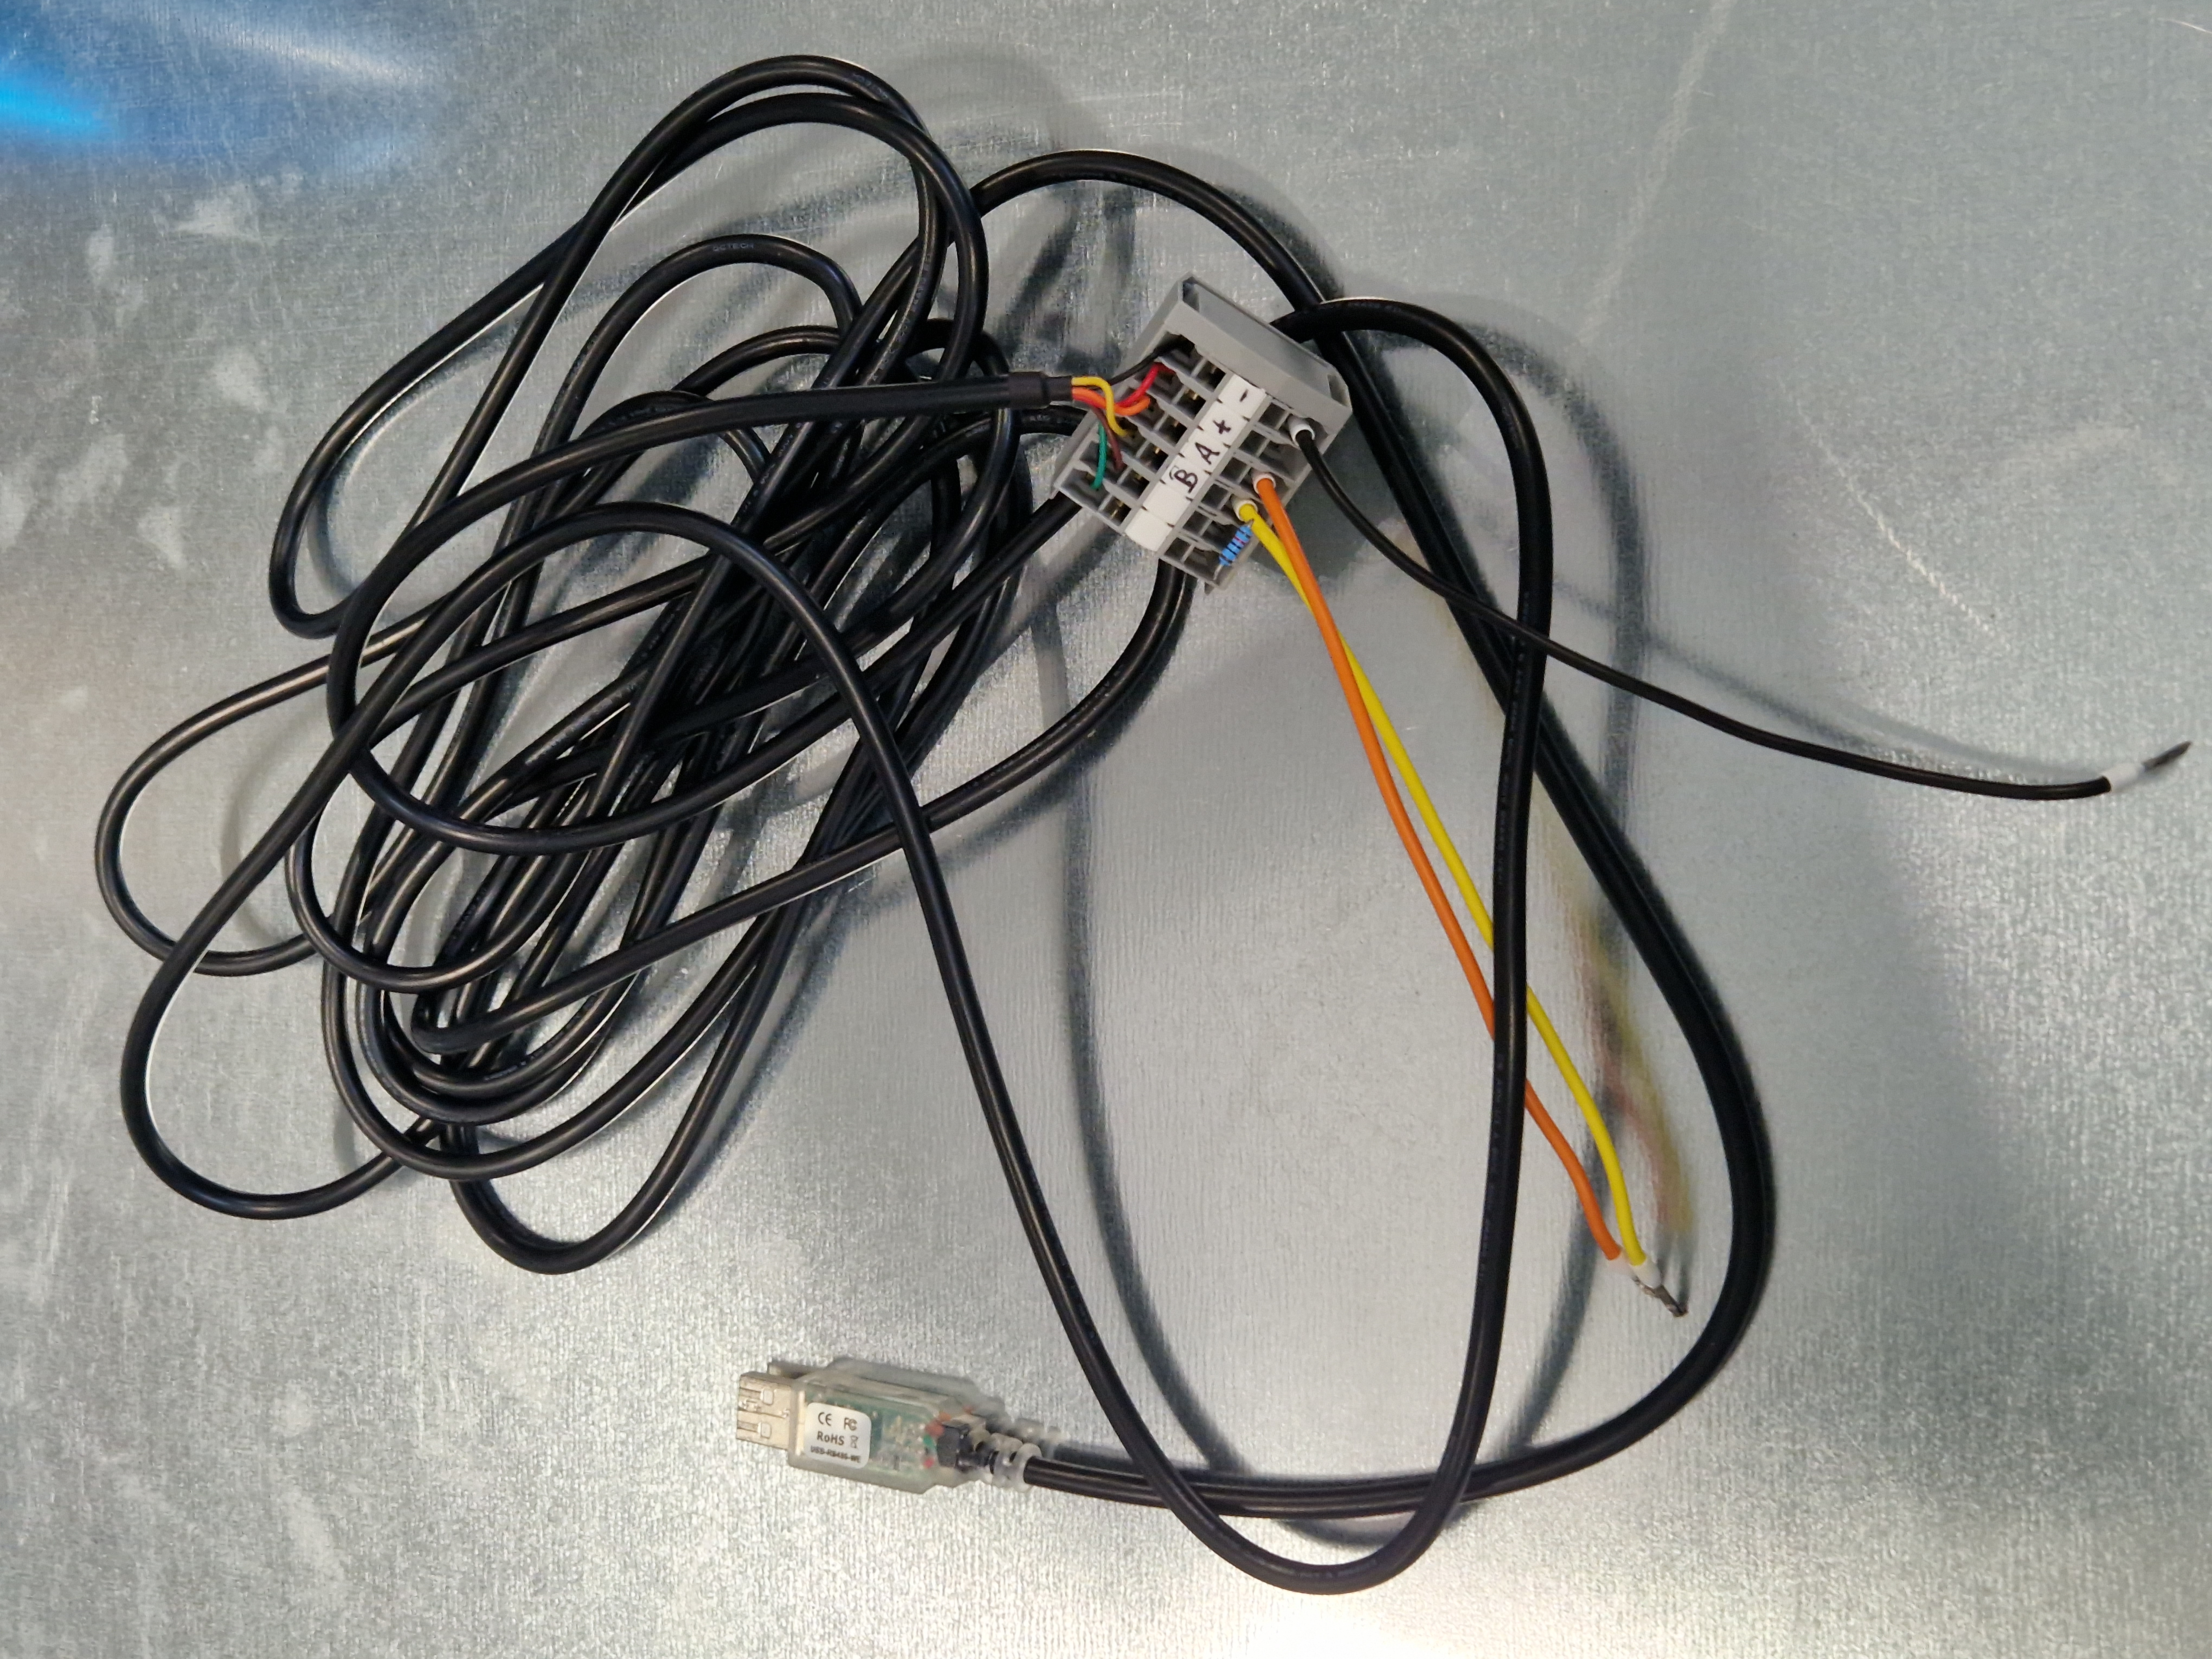
\includegraphics[width=0.5\linewidth]{Bilder/modbus_usbkabel}
	\caption{Modbus USB-Kabel} 
	\label{fig:modbus_usbkabel}
\end{figure}

 Danach werden die Einzelnen Komponenten der seriellen Kommunikation angegeben:
\begin{itemize}
	\item Baudrate (9600)
	\item Parity (Even)
	\item Stop Bits (1)
	\item Node Adresse (2)
	\item Starting Address 1 (Register fängt bei eins an und ist in nicht in Hexadezimal angegeben)
	\item Length To Read (Die ersten 85 Werte sollen ausgegeben werden)
	\item Read Funktion (FC 3 - Holding Register)
\end{itemize}

Beschreibung der Werte und Funktion von: Baudrate, Parity, Stop Bits, Read Funktion siehe \ref{modbus_funktionsweise}.



Abb.~\ref{fig:Shortbusausgabe}. 

\begin{figure}[H]
	\centering
	\includegraphics[width=1\linewidth]{Bilder/shortbus_ausgabe}
	\caption{Shortbus in Entwicklungsphase} 
	\label{fig:Shortbusausgabe}
\end{figure}


\subsection{VOR ABGABE LÖSCHEN}
%Umsetzung von Shortbus
%allgemein was kann das programm:

%wie lese ich daten aus
%das tdot / entwicklungsgerät 

\section{Hardware-Evaluation und -Selektion}
\setAuthor{\mangeng}
\subsection{Evaluierung} \label{evaluierung}
Damit die Ausarbeitung beginnen kann, muss eine gute Kombination für die zukünftigen Hardware-Komponenten zusammengestellt werden. Diese Kombination sollte auf den Spezifikationen basieren, die vom Projektbetreuer Simon Köldorfer definiert wurden. Diese Spezifikationen umfassen die grundsätzliche Verwendung eines Displays, die IP66-Tauglichkeit des Gehäuses, die Witterungstauglichkeit der Anzeige sowie die Möglichkeit, die Anzeigeseite zu ändern, wobei nicht spezifiziert ist, wie dies umgesetzt werden soll. Die Spannungsversorgung muss außerdem als 24V AC/DC ausgeführt sein. Schließlich sollte die Lösung auch wirtschaftlich sinnvoll sein, falls das Unternehmen entscheidet, diese Anzeige fortan an mehreren oder sogar allen Lüftungsgeräten anzubringen. Die genaueren Spezifikationen befinden sich im Kapitel \ref{aufgabenstellung}.\\
Trotz dieser Definitionen blieb genug Freiheit, um mehrere Möglichkeiten zusammenzustellen und somit dem nachzugehen, was für diese Diplomarbeit am passendsten ist. 
Folgend werden alle vier Varianten gelistet, die später auch so innerhalb eines Meetings dem Projektbetreuer näher gebracht wurden. \\
Allgemein zu sagen ist, dass die angegebenen Preise möglicherweise von der Realität etwas abweichen können. Auch, dass die Schwierigkeit der Umsetzungen jeweils bei einem akzeptablen Level liegt und bei allen Varianten die Terminierung oder die Weiterleitung des Modbus-Signals ein Problem sein könnte.
\paragraph{Variante A}
Die erste Variante beinhaltet als einzige den Mikrocontroller Arduino. Genauer gesagt handelt es sich um den Arduino Mega. Unter Abbildung \ref{fig:arduino_mega} findet man eine Darstellugn davon. Bei dieser Variante ist die Grundidee, ein kleines 3.5-Zoll Display mit 1-2 Buttons herzustellen und alles in einer IP66 tauglichen, kleinen Box zu verstauen. 
Die positiven Aspekte dieser Variante beziehen sich sowohl auf den Preis als auch auf die Verfügbarkeit der Teile. Variante A hat mit Abstand den niedrigsten Gesamtpreis, dieser liegt bei ungefähr 63,00€ und die Verfügbarkeit ist stets gegeben. Auch die Haltbarkeit ist ein positiver Aspekt, da jegliche Witterungen dem Gehäuse nichts ausmachen, und im Fall, dass es doch kaputtgeht, es leicht und günstig zu ersetzen ist. Schwierigkeiten existieren jedoch beispielsweise bei der Benutzerfreundlichkeit, da die Bedienung mit 2 Buttons komplizierter bzw. umfangreicher ist als mit einem. Auch bei den Dokumentationen mangelt es etwas, denn während ausreichend Dokumentationen über die Hardware zur Verfügung steht, sind die Dokumentationen über die Software bzw. über die Libraries eher kurz gehalten, wie beispielsweise bei der Library \enquote{ModbusMaster}.
\begin{figure}[ht]
	\centering
	\includegraphics[width=0.5\linewidth]{Bilder/ARDUINO_MEGA.jpg}
	\caption{Arduino Mega (Quelle: \url{https://cdn-reichelt.de/bilder/web/artikel_ws/A300/ARDUINO_MEGA_01_NEU.jpg})}
	\label{fig:arduino_mega}
\end{figure}
\paragraph{Variante B}
Variante B hat als Grundkonzept ein 7-Zoll-Display, welches nicht berührungsempfindlich ist und auch nicht wasserfest, und deswegen wie in Variante A in eine witterungsfeste Box gelegt und durch Buttons gesteuert wird. Neben den unterschiedlichen Bildschirmgrößen unterscheidet auch der verwendete Mikrocontroller die beiden Kombinationen, denn hier wird ein Raspberry PI als Zentralrechner etabliert. Eine Abbildung davon ist in Abbildung \ref{fig:raspi3} zu sehen.\\
Der Gesamtpreis der Hardware liegt bei ungefähr 93.00€ und ist somit auch noch eine der günstigeren Versionen. Für diese Variante sprechen aber noch andere Faktoren. Einerseits die erhöhte Benutzerfreundlichkeit im Vergleich zur Variante A, denn auch wenn wieder Buttons für die Navigation verwendet werden, erleichtert das größere Display die Übersicht. Andererseits die Witterungsfestigkeit aufgrund des Gehäuses, welches bei Schäden leicht und günstig zu ersetzen ist. Auch Dokumentationen sind ausreichend für Hardware und Software vorhanden. Die Probleme hierbei beziehen sich jedoch auf die Verfügbarkeit des Raspberry PIs, da diese in letzter Zeit entweder wenig verfügbar oder teuer sind. Der Display-Preis ist zwar auch nicht niedrig, kann aber durch Mengenrabatte reduziert werden.
\begin{figure}[ht]
	\centering
	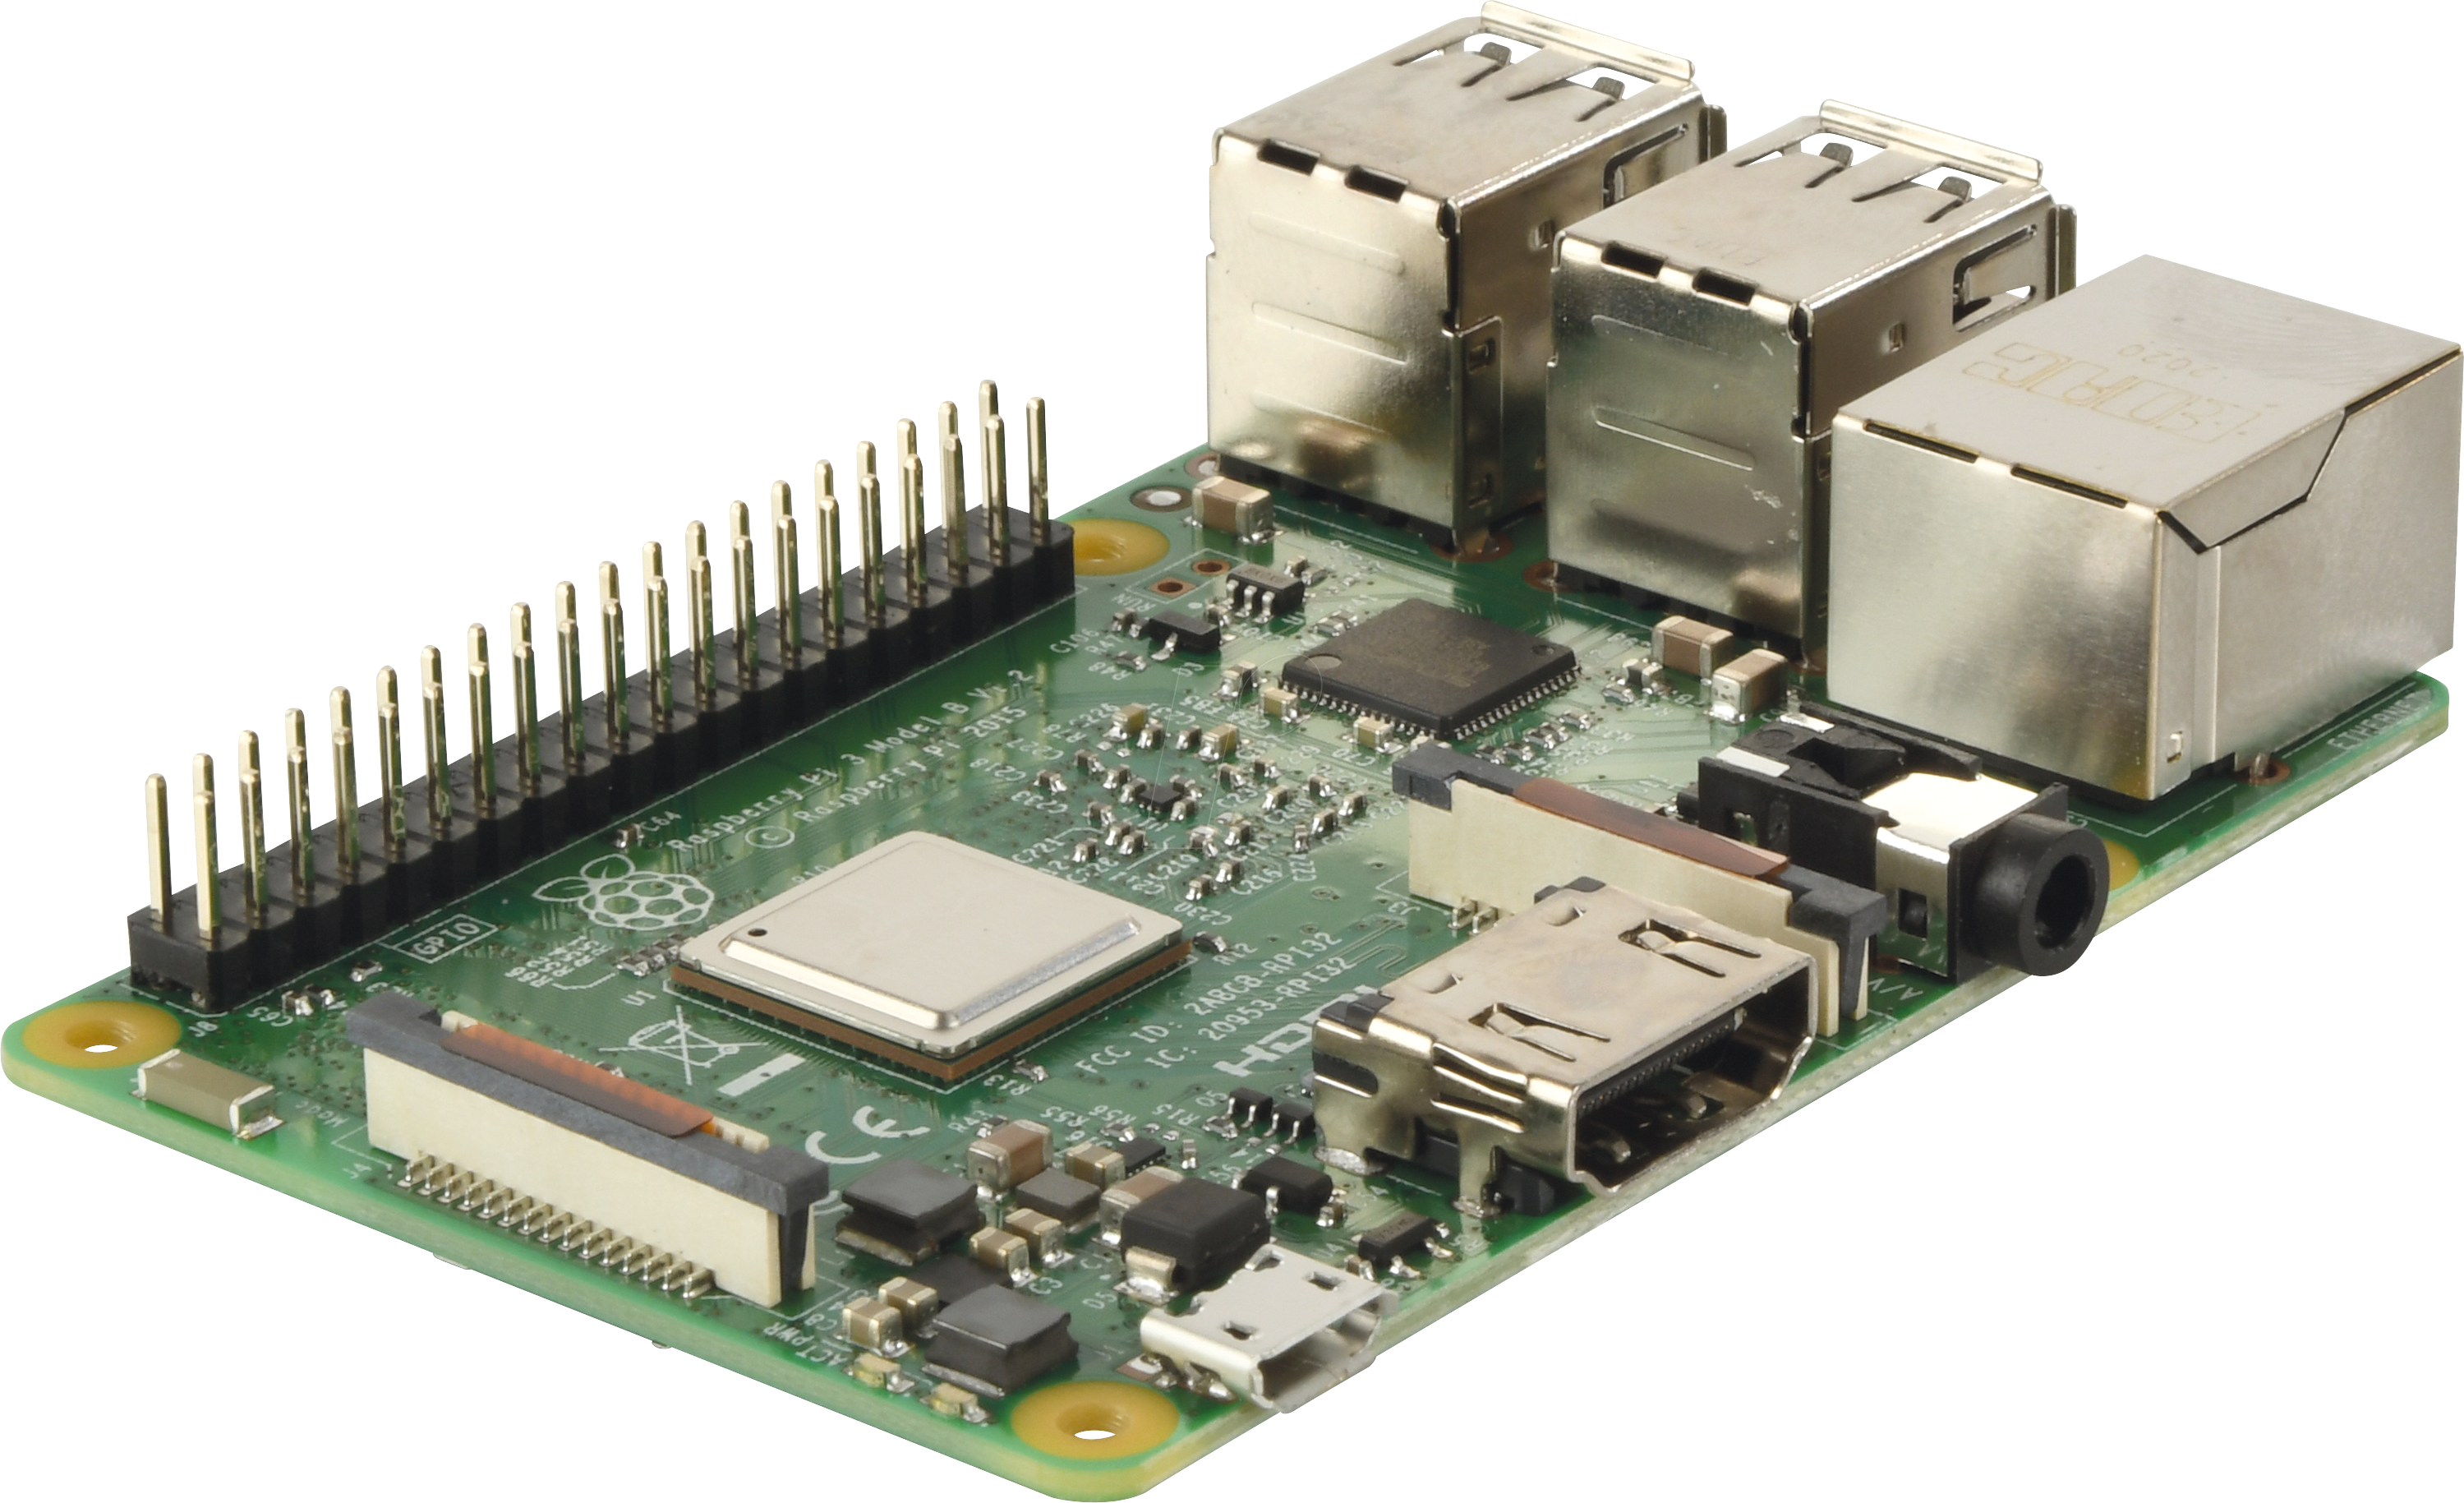
\includegraphics[width=0.6\linewidth]{Bilder/RASPBERRY_PI3.png}
	\caption{Raspberry PI 3 (Quelle: \url{https://cdn-reichelt.de/bilder/web/xxl_ws/A300/RASPBERRY_PI_3_02_20210420.png})}
	\label{fig:raspi3}
\end{figure}
\paragraph{Variante C}
Die dritte Variante ist die mit Abstand teuerste, denn hier liegt der Preis bei etwa 117,00€. Der Grund dafür ist, dass die Konzeption aus einem \gls{kapazitiv}n 7-Zoll-Display besteht. Dieses wird unter Abbildung \ref{fig:kapazitives_display} abgebildet. Neben der eigentlich nicht gegebenen Witterungsfestigkeit des Displays per se, wird es jedoch so verbaut, dass diese Eigenschaft trotzdem gegeben ist. Dennoch kann sich möglicherweise die Handhabung der Touchfunktion mit der Zeit aufgrund fehlender Wasserfestigkeit verschlechtern. Da auch hier wieder der Raspberry PI die Grundlage des Systems spielt, ist auch wieder die Verfügbarkeit dessen unpassend. Positive Aspekte sind allgemein die Touchfunktion, da diese weit verbreitet ist und die Bedienung für den Nutzer einfach hält. Ebenso gibt es ausreichend Dokumentationen für Hardware und Software, trotzdem kann die Implementation der Touch-Funktion Probleme bereiten.
\begin{figure}[ht]
	\centering
	\includegraphics[width=0.6\linewidth]{Bilder/kapazitives_display.jpg}
	\caption{\gls{kapazitiv}s Display (Quelle: \url{https://www.berrybase.at/media/image/49/8e/36/ID_53172_orig_600x600.jpg})}
	\label{fig:kapazitives_display}
\end{figure}
\newpage
\paragraph{Variante D}
Die vierte und letzte Variante charakterisiert sich durch eine weitere Nutzung eines \gls{kapazitiv}n oder diesmal auch \gls{resistiv}n 7-Zoll-Displays, welches nicht wasserdicht ist. Der Zugriff zum Display erfolgt durch eine transparente Klappe am Gehäuse. Eine Abbildung dieses Gehäuses befindet sich unter Abbildung \ref{fig:gehäuse_mit_klappe}. Auch hier wird der Raspberry PI als Mikrocontroller verwendet, welches auf zuvor genannte Probleme bezüglich der Verfügbarkeit zurückführt. Das Display zu erhalten führt zu keinen Schwierigkeiten und man erhält auch wieder einen Mengenrabatt. Nichtsdestotrotz liegt der Gesamtpreis bei ungefähr 108,00€ und ist somit eine der teureren Zusammenstellungen. Dafür stellen Witterungsprobleme keine Erschwernisse dar, solange nicht vergessen wird, die Klappe am Gehäuse immer ordnungsgemäß zu schließen. Die Situation mit den Dokumentationen ist äquivalent zu Variante B und C und somit auch kein Problem. Zurückkehrend auf die unterschiedlichen Displays: Die \gls{kapazitiv} Version hat eine allgemein besser funktionierende Touch-Funktion, die aber durch nasse Hände genommen wird und somit die Nutzung bei beispielsweise Regen erschwert wird. Die \gls{resistiv} Version ermöglicht dafür eine besseren Reaktionsfähigkeit bei nassen Händen oder sogar beim Tragen von Handschuhen.
\begin{figure}[ht]
	\centering
	\includegraphics[width=0.6\linewidth]{Bilder/gehäuse_klappe.png}
	\caption{Gehäuse mit Klappe (Quelle: \url{https://asset.conrad.com/media10/isa/160267/c1/-/de/706888_BB_00_FB/image.jpg?x=1000&y=1000&format=jpg&ex=1000&ey=1000&align=center})}
	\label{fig:gehäuse_mit_klappe}
\end{figure}
\newpage
\paragraph{Bewertungsmatrix}

Um eine umfassende Übersicht über die potenziell verfügbaren Varianten sowie ihre spezifischen Merkmale sicherzustellen, wurde eine detaillierte Bewertungsmatrix in Excel erstellt. Diese Matrix befindet sich auf der nächsten Seite unter Abbildung \ref{fig:matrix}.
\begin{landscape}
	\begin{figure}[H]
		\centering
		\includegraphics[width=1\linewidth]{Bilder/bewertungsmatrix}
		\caption{Bewertungsmatrix der Hardwarekomponente}
		\label{fig:matrix}
	\end{figure}
\end{landscape}

\setAuthor{\fenkart}
\newpage
\subsection{Selektion} \label{selektion}
Die im Kapitel \ref{evaluierung} auf der Grundlage der Recherche erstellten Varianten mussten während eines Meetings dem Projektleiter und einer externen Person präsentiert werden. Ziel war es, die Varianten zu analysieren und festzustellen, welche für die praktische Umsetzung sinnvoll sind und auch wirtschaftlich vertretbar erscheinen. Im Folgenden befindet sich eine kurze Beschreibung der jeweiligen Varianten in Kombination mit den im Meeting angemerkten Punkten.

\begin{itemize}
	\item \underline{Variante A:} Hier ist ein etwas kleineres Display in Verwendung, genauer gesagt ein 3.5-Zoll-Display, mit einem Chipsatz, der anders als bei den anderen Varianten ist, nämlich der Arduino Mega. Für diese Umsetzung muss eine Platine zwischen Display und Board erstellt werden für die Pins, demnach ist es nicht besonders effizient erweiterbar wie beispielsweise bei dem Raspberry Pi. Bei dieser Version wird alles in einem IP66 geschützten Gehäuse verbaut und mit Buttons gesteuert. Laut Simon Köldorfer sei diese Methode sinnvoller und einfacher als bei der Nutzung eines Touchscreens, da dieser zu viele Funktionen für eine schlichte Anzeige habe und auch nicht sehr geeignet für bestimmte Wetterkonditionen sei. \\
	Aufgrund der begrenzten Verfügbarkeit von Libraries für die Benutzeroberfläche auf dem Arduino wird das Erscheinungsbild mit der vom Projektteam ausgewählten Library weniger ansprechend sein. Diese Library bietet lediglich die Möglichkeit, mit Texten, Rechtecken, Linien und Kreisen eine Benutzeroberfläche zu kreieren.
	\item \underline{Variante B:} Diese Kombination an Hardware-Komponenten ist der Favorit des Projektteams. Hier wird ein größeres Display mit 7-Zoll und einem Raspberry Pi 3 als Chipsatz verwendet. Die Gesamtheit wird wieder in einer IP66-tauglichen Box verstaut. Diese Variante ist zwar teurer als die erste, dafür kann die Umsetzung schöner realisiert werden. Auch kann man sich die RS323-Schnittstelle sparen, da man stattdessen einen USB-Port zur Verfügung hat.
	\item \underline{Variante C:} Variante C ist gleich zu Variante A, nur dass ein Touchdisplay implementiert wird, wodurch auch Einsparungen am Gehäuse erfolgen. Diese Einsparung kann jedoch zu Problemen mit bestimmten Witterungen wie zu starker Sonneneinstrahlung, Regen, usw. führen. 
    Es gibt zwar auch andere, widerstandsfähigere Industriedisplays, diese sind aber auch deutlich teurer und bereits ohne das handelt es sich hier um die teuerste Variante, die zusätzlich nicht wasserfest ist.
	\item \underline{Variante D:} Hier handelt es sich um dasselbe Konzept wie in Variante C, nur dass eine Klappe implementiert ist. Diese muss immer geöffnet werden, wenn durch die Werte gescrollt werden will, was nicht sehr praktisch ist, da diese bei zu öfter Verwendung kaputtgehen kann. Auch ist hier die Witterung wieder ein Thema, da das Display bei Regen beispielsweise durch die nicht vorhandene Wasserfestigkeit einen Schaden erhalten kann.
\end{itemize}

\paragraph{Endgültige Entscheidung}
Die Entscheidung gegen die Varianten C und D wurde aufgrund der unnötig komplizierten Handhabung des Touchdisplays, der erhöhten Fehleranfälligkeit und der damit verbundenen hohen Kosten getroffen. \\
Für Variante A wurde angemerkt, dass die einfache Darstellung der Werte möglicherweise nicht ästhetisch ansprechend wäre. Allerdings wurde darauf hingewiesen, dass die Herstellung der Platine von einem derzeitigen Ferialpraktikanten der HTL Rankweil durchgeführt werden könnte. \\
Bezüglich Variante B wurde festgestellt, dass die Umsetzung auch mit einem Raspberry Pi Zero möglich wäre, was zusätzliche Kosteneinsparungen bedeutet. Da der Raspberry Pi zudem erweiterbar ist und diese Version ein größeres Display verwendet, fiel die Entscheidung auf diese Variante.


\section{Software-Selektion}
\setAuthor{\schneider}
Für die Ausarbeitung der Diplomarbeit stehen eine Vielzahl von Programmiersprachen zur Verfügung. Geachtet wurde bei der Auswahl auf die Einfachheit bzw. Vertrautheit der einzelnen Teammitglieder mit der Sprache, deren Funktionalität, das Bibliotheken-Angebot und die vorhandene Dokumentation. In dieser Diplomarbeit wird somit die Programmiersprache Python verwendet. Auf die genauen Gründe zur Auswahl wird in dem folgenden Kapitel \ref{python_kapitel} eingegangen.

\subsection{Python}\label{python_kapitel}
\begin{minipage}{0.6\textwidth}
	Python ist eine vielseitig einsetzbare Programmiersprache. Die Erstellung einer ersten Version wurde 1989 von Guido van Rossum als Hobbyprojekt gestartet, während er am Centrum Wiskunde \& Informatica Institut in den Niederlanden arbeitete. Diese erste Version erschien 1991. Seither wird Python stetig weiterentwickelt. Besonders durch seine einfache Syntax und die vielen vorhandenen Bibliotheken konnte sich Python immer stärker auch in betrieblichen Umgebungen etablieren. Im Gegensatz zu Sprachen wie C, C\#, etc. verwendet Python keinen Compiler, um das Coding vor der Ausführung des Programms in Maschinencode umzuwandeln, sondern einen Interpreter, der beim Start des Programms jede Zeile nacheinander überprüft und ausführt. Diese Praktik wurde erstmals mit der Programmiersprache Lisp eingeführt und wird unter anderen von Java, Ruby oder PHP benutzt. 
	\cite{Python_Software_Foundation:o.J., Pramanick_gfg:2019, Ryte:2021}
\end{minipage}%
\hfill
\begin{minipage}{0.37\textwidth}
	\centering	
	\includegraphics[width=0.58\textwidth]{Bilder/Python_logo}
	\captionof{figure}{Python Logo (Quelle:\\
		\url{https://en.wikipedia.org/wiki/File:Python-logo-notext.svg}) \label{fig:python_logo}}
\end{minipage}
\vspace{1ex}

Die folgenden Vor- und Nachteile beziehen sich auf \textcite{Ceaseo:2020}.
\paragraph{Vorteile}
\begin{itemize}
	\item Nicht nur die Syntax ist übersichtlich, sondern auch die Bibliotheken-Verwaltung ist einfach. Mit dem pip-Paketmanager können mit einem \enquote{pip install} alle vorhandenen Bibliotheken installiert werden.
	\item Python kann in den unterschiedlichsten Anwendungen zum Einsatz kommen. Es können damit unter anderem Web-, Mobile- und Backendanwendungen erstellt werden. Außerdem eignet sie sich auch als Skriptsprache für Probleme, bei denen es keiner komplexen Software bedarf. Es können objektorientierte Strukturen genauso wie funktionale verwendet werden. 
	\item Wie bereits erwähnt, bietet Python sehr viele unterschiedliche Bibliotheken, die von der Community ständig weiterentwickelt und verbessert werden. Außerdem besitzen diese Bibliotheken meist gut angelegtes Dokumentationsmaterial und Diskussionen bzw. Hilfestellungen in diversen Foren.
\end{itemize}

\paragraph{Nachteile}
\begin{itemize}{}{}
	\item Da die Sprache Zeile für Zeile interpretiert wird, dauert die Ausführung länger als bei kompilierten Sprachen.
	\item Zur Initialisierung einer Variable muss kein Datentyp angegeben werden. Dadurch hat der Programmierer weniger Schreibaufwand, allerdings können in erhöhtem Maße Laufzeitfehler auftreten und auch die Übersichtlichkeit ist betroffen. Genauso ist die Abwesenheit von Klammern eine kontroverse Funktionalität.
\end{itemize}

\paragraph{Gründe für die Verwendung}
Ein ausschlaggebender Grund für die Verwendung von Python ist, dass alle Teammitglieder damit schon Erfahrungen gemacht haben. Beim Einsatz anderer Sprachen wäre die Einarbeitungszeit einzelner Teammitglieder zu berücksichtigen. Außerdem liegt es nahe, da es für den Raspberry PI eine Standardsprache ist. Die oben beschriebenen Nachteile der Sprache sind für ein Proof-of-Concept vernachlässigbar. Außerdem hat die Recherche ergeben, dass viele gut dokumentierte Bibliotheken für Modbus und \aclp{gui} vorhanden sind.

\paragraph{Verwendete Python-Bibliotheken}
Für das Auslesen der \acfp{rlt} Messwerte über das Modbus Protokoll wird minimalmodbus verwendet. Um die erhaltenen Werte auch grafisch anzuzeigen, wird CustomTkinter verwendet. Es folgen die Beschreibungen dieser beiden Bibliotheken.


\setAuthor{\pezze}
\subsection{\acs{json} und \acs{csv}}
\paragraph{Was ist \acs{csv}?}
\acf{csv} ist ein systemunabhängiges Format für Textdateien. \acs{csv} Dateien dienen zum Speichern und Übertragen von strukturierten Daten, hauptsächlich Tabellen oder Listen, wobei durch die Verkettung von mehreren \acs{csv} Dateien oder mithilfe von zusätzlichen Regeln auch geschachtelte Objekte gespeichert werden können. \cite{Fuchs Media Solutions:o.J.}

Die erste Verwendung des Datenformates geht auf 1972 zurück, wo es vom IBM FORTRAN IV (H Extended) Compiler unterstützt wurde. Trotzdem gibt es gegenwärtig für CSV keinen allgemeinen Standard, wobei aber mit dem RFC 4180 Dokument \cite{Shafranovich:2005} im Jahre 2005 ein erster Versuch einer weit verbreiteten inoffiziellen Definition existiert. Dieses Dokument besagt:
\begin{list}{}{}
	\item Hi
	\item 123ljö
\end{list}

\chapter{Umsetzung}

\section{Raspberry PI Aufsetzung}
\setAuthor{\pezze}
\label{raspi_setup}
In diesem Kapitel werden kurz die erforderlichen Schritte erläutert, um einen Raspberry PI zur Entwicklung der \ac{rltanzeige} aufzusetzen.
Zur Entwicklung der Diplomarbeit wurden unterschiedliche Versionen des Raspberry PIs genutzt (Raspberry PI 3 Modell B, Raspberry PI Zero). Dabei kommt als Betriebssystem Raspberry PI OS (Version 11 \enquote{bullseye}) zum Einsatz, welches leicht adaptiert wird.

\subsection{Headless Setup}\label{raspi_headless_setup}
Während der Entwicklung der \ac{rltanzeige} wird mit mehreren Raspberry PIs gearbeitet, die nicht alle gleichzeitig an einem externen Bildschirm angeschlossen werden können. Außerdem verfügt das Raspberry PI Zero Modell aufgrund seiner geringen Größe nur über einen Mini-\ac{hdmi} Anschluss, wofür ein spezielles Kabel \bzw ein spezieller Adapter benötigt wird, und somit nicht einfach ein externer Bildschirm angeschlossen werden kann. Daher wird ein sog. \enquote{Headless Setup} notwendig, bei dem der Raspberry PI ohne angeschlossenen Bildschirm, Tastatur oder Maus gestartet werden kann. Mittels \ac{ssh} oder \ac{vnc} Client kann dann auf den Raspberry PI zugegriffen werden.
\cite[vgl.][]{Piltch:2022}

\paragraph{Aktivierung von \textit{SSH}}
\ac{ssh} ist ein Netzwerkprotokoll, das verwendet wird, um sich sicher über das Netzwerk mit einem anderen Gerät zu verbinden und darauf Operationen auszuführen. \ac{ssh} ist am Raspberry PI standardmäßig deaktiviert.  Daher muss \ac{ssh}, durch das Erstellen einer Datei Namens \enquote{ssh.} auf der SD-Karte, aktiviert werden. Nun kann eine kabellose oder kabelgebundene \ac{ssh} Verbindung mit dem Raspberry PI aufgebaut werden.

\paragraph{Kabellose Verbindung über \textit{SSH}}
Für eine kabellose Verbindung über \ac{ssh} muss zuerst auf dem Raspberry PI ein Netzwerkzugang konfiguriert werden. Dazu wird auf der SD-Karte eine Konfigurationsdatei Namens \enquote{wpa\_supplicant.conf} mit folgendem Inhalt angelegt:
\begin{textcode}
country=DE
ctrl_interface=DIR=/var/run/wpa_supplicant GROUP=netdev
update_config=1

network={
    scan_ssid=1
    ssid="[SSID]"
    psk="[Passwort]"
}
\end{textcode}

Nach dem ersten Start lässt sich nun der Raspberry PI mit dem folgenden Befehl über die Kommandozeile verbinden:
\begin{minted}{console}
ssh [Username]@[IP-Adresse]
\end{minted}

\paragraph{Kabelgebundene Verbindung über \textit{SSH}}
Da die normale Version des Raspberry PI Zero keine kabellose Netzwerkverbindung unterstützt, ist es notwendig, eine kabelgebundene Verbindung herzustellen, um \ac{ssh} zu verwenden. Dazu sind folgende Schritte notwendig:

\begin{enumerate}
    \item Am Ende der Datei \enquote{config.txt} auf der SD-Karte folgende Zeile hinzufügen: \begin{textcode}
    dtoverlay=dwc2.
    \end{textcode}
    \item In der Datei \enquote{cmdline.txt} nach \enquote{rootwait} folgendes einfügen:
    \begin{textcode}
    modules-load=dwc2,g_ether
    \end{textcode}
    \item Den Raspberry PI Zero über USB mit einem Computer verbinden, wobei am Raspberry PI der Daten-USB-Anschluss verwendet werden muss und nicht der Strom-USB-Anschluss.
    \item Apple Bonjour-Druckdienste auf dem Windows Computer herunterladen.
    \item Nun lässt sich nun der Raspberry PI mit dem folgenden Befehl über die Kommandozeile verbinden:
    \begin{minted}{console}
ssh [Username]@[RaspberryPIZero-Name].local
    \end{minted}
\end{enumerate}

\subsection{Installieren der nötigen Python Pakete}
Nach dem Aufsetzen des Raspberry PI OS und \ac{ssh} müssen zuletzt noch die Python Pakete für \gls{gls_tk}, \gls{gls_ctk} und \gls{gls_minimalmodbus} mit den folgenden Befehlen auf dem Raspberry PI installiert werden:

\begin{minted}{console}
pip install tk
pip install customtkinter
pip install minimalmodbus
\end{minted}


\setAuthor{\mangeng}
\input{library_installation}

\section{\acf{gui}}\label{gui_design}
\setAuthor{\pezze}
\subsection{Figma Design}\label{figma_design}
\begin{minipage}{0.6\textwidth}
    Zur Erstellung eines Mockup des Designs für die \acs{gui} der \acs{rltanzeige} wurde Figma verwendet. Figma Design ist eine Applikation zum Erstellen von Prototypen im Bereich \ac{uxui}. Dabei kann im Team in Echtzeit zusammen gearbeitet werden. Mit Figma können in das erstellte Design direkt interaktive Funktionen eingebaut werden, um ein realistisches Prototyping zu ermöglichen. Ein weiterer Vorteil von Figma ist der sog. \enquote{Dev Mode}. Mit diesem können Entwickler direkt auf das Design zugreifen und Details finden, die benötigt werden, um das Design in Code umzusetzen. \cite[vgl.][]{figma_design:o.J.}
\end{minipage}%
\hfill
\begin{minipage}{0.37\textwidth}
	\centering	
	\includegraphics[width=0.50\textwidth]{figma_logo}
	\captionof{figure}{Figma Logo (Quelle: 
		\url{https://en.m.wikipedia.org/wiki/File:Figma-logo.svg}) \label{fig:figma_logo}}
\end{minipage}
\vspace{1ex}

Bei Erstellung des Designs für die \acs{rltanzeige} liegt die Priorität auf Übersichtlichkeit und guter Leserlichkeit. Die Wahl eines $3,5$ Zoll Displays hätte (mit ausreichender Übersichtlichkeit) lediglich die simultane Darstellung von maximal $2$ Werten erlaubt. Die tatsächliche Wahl eines $7$ Zoll Displays zur Anzeige ermöglicht hingegen die zeitgleiche Darstellung mehrerer Werte, wobei $5$ bis $6$ Werte den idealen Kompromiss zwischen genug Information und Übersichtlichkeit bieten. Um die Übersichtlichkeit weiter zu erhöhen ist die Kategorisierung der Messwerte in sinnvolle und zusammenhängende Seiten wichtig. Alle Informationen zu wichtigen Temperaturen sollen beispielsweise auf einer Seite gruppiert sein, während alle Informationen zu einem bestimmten Ventilator auf einer anderen Seite zu finden sind. Hierbei benötigt jede jeweilige Seite eine Überschrift zur Orientierung. Zusätzlich sollte es eine Indikation geben, die der Nutzerin oder dem Nutzer signalisiert, auf welcher Seite sie oder er sich gerade befindet. Tasten zum Seiten wechseln werden nicht benötigt, da an der \acs{rltanzeige} zwei physikalische Knöpfe verbaut sind.

\begin{figure}[H]
    	\begin{subfigure}[t]{0.5\textwidth}
    		\centering
    		\frame{\includegraphics[width=0.99\textwidth, page=1]{design_varianten}}
    		\caption{Design Variante A \label{fig:variante_a}}
    	\end{subfigure}
        \hfill
    	\begin{subfigure}[t]{0.5\textwidth}
    		\centering
    		\frame{\includegraphics[width=0.99\textwidth, page=2]{design_varianten}}
    		\caption{Design Variante B \label{fig:variante_b}}
    	\end{subfigure}
    \begin{subfigure}[t]{\textwidth}
		\centering
		\frame{\includegraphics[width=0.70\textwidth, page=3]{design_varianten}}
		\caption{Design Variante C \label{fig:variante_c}}
	\end{subfigure}
	\caption{\acs{gui} Design Varianten \label{fig:design_varianten}}
\end{figure}

Mit den zuletzt genannten Kriterien wurden drei Designvarianten entworfen (siehe Abb. \ref{fig:design_varianten}). Zur Umsetzung gelangte schlussendlich Variante C (siehe Abb. \ref{fig:variante_c}). Diese bietet mit dem Kontrast im Hintergrund jedes einzelnen Messwerts und der listenartigen Aufzählung die besten Eigenschaften, um Messwerte auf einem Display mit begrenzter Auflösung und Helligkeit in Umgebungen mit suboptimalen Bedingungen ablesen zu können. 


\subsection{Umsetzung der GUI im Code}\label{tkintercode}
\paragraph{Klassenstruktur}
Im Vordergrund basiert die Klassenstruktur grundsätzlich auf \gls{gls_ctk} Komponenten (siehe Abb.~\ref{fig:klassenstruktur_frontend}). Dabei gibt es die Klassen \enquote{App}, \enquote{PageFrame}, \enquote{TitleFrame} und \enquote{MeasurementFrame}. Im Programm wird eine \enquote{App} Instanz ausgeführt, welche das Hauptfenster ist. Diese Instanz kann beliebig viele \enquote{PageFrames} enthalten, die wiederum jeweils ein \enquote{TitleFrame} und eine Liste von \enquote{MeasurementFrames} beinhalten. Die \enquote{PageFrames} stellen die einzelnen Seiten dar, welche per Knopfdruck an der \acs{rltanzeige} durchgeblättert werden können. In einem \enquote{TitleFrame} wird immer der Titel der jeweiligen Seite gespeichert \bzw angezeigt. In den \enquote{MeasurementFrame} Instanzen werden hingegen die tatsächlichen Messwerte (Bezeichnung + Wert + Maßeinheit) dargestellt.

\begin{figure}[H]
	\centering
	\includegraphics[width=0.95\textwidth]{uml_frontent_class_diagram}
	\caption{UML Diagramm Frontend \label{fig:klassenstruktur_frontend}}
\end{figure}

\paragraph{CustomTkinter Code}
Eine nähere Beschreibung und die Umsetzung der vorher genannten Klassen erfolgt in diesem Kapitel. 
\newline Wie zuletzt beschrieben, basieren alle Klassen im Frontend auf \gls{gls_ctk}. Die Klassen sind dabei alle (bis auf die Klasse \enquote{App}) vom Typ \enquote{CTkFrame}. Ein \enquote{CTkFrame} ist ein Widget, das wie ein Rahmen \bzw Behälter für andere Widgets fungiert. So können diese in weiteren Widgets gruppiert und besser organisiert werden. Als erster Parameter wird für \enquote{CTkFrames}, wie bei allen \gls{gls_tk} und \gls{gls_ctk} Widgets, der \enquote{master} \bzw das Elternobjekt angegeben. Darüber hinaus können die Breite (\enquote{width}), Höhe (\enquote{height}), Rahmenbreite \bzw -Farbe (\enquote{border\_width} \bzw \enquote{border\_color}) sowie die Hintergrundfarbe (\enquote{fg\_color}) angegeben werden. \cite[vgl.][]{Schimansky:o.J.}

Die Klasse \enquote{TitleFrame} enthält ein \enquote{CTkLabel}, welches mit der \enquote{place( )} Methode im Behälter platziert wird. Die Klasse \enquote{CTkLabel} basiert auf der Klasse \enquote{tkinter.Label} und dient zur Darstellung eines Textes. Im \enquote{TitleFrame} Label steht immer der Titel der zugehörigen Seite. Das \enquote{title\_font} Objekt, welches im folgenden Code zu sehen ist, ist eine Instanz der \gls{gls_ctk} Utility Klasse \enquote{CTkFont}. Es wird verwendet, um die Schriftformatierung von \gls{gls_ctk} Widgets vorzunehmen. Jedes \gls{gls_ctk} Widget bekommt standardmäßig ein \enquote{CTkFont} Objekt, wobei ein solches Objekt zeitgleich mehreren Widgets angefügt werden kann. Eine Änderung eines \enquote{CTkFont} Objekts wird an alle Widgets, die es verwenden, weitergeleitet. \cite[vgl.][]{Schimansky:o.J.}

\begin{pythoncode}
class TitleFrame(ctk.CTkFrame):
	def __init__(self, master, title, **kwargs):
		super().__init__(master, width=800, height=60, fg_color=text_color, **kwargs)
		
		title_font = ctk.CTkFont(family="Roboto", size=32)
		
		self.title_lbl = ctk.CTkLabel(master=self, text=title, width=700, height=45, fg_color="transparent", text_color=title_color, anchor=ctk.CENTER, font=title_font)
		self.title_lbl.place(relx=0.5, rely=0.12, anchor=ctk.N)
\end{pythoncode}

Wie in der Klassenstruktur beschrieben, beinhaltet ein jedes \enquote{PageFrame} neben einem \enquote{TitleFrame} eine Liste von \enquote{MeasurementFrames}. Eine Instanz der Klasse \enquote{MeasurementFrame} enthält immer Informationen zu einem bestimmten Messwert, welche mithilfe von zwei \enquote{CTkLabel} Widgets dargestellt werden. Dabei wird die Bezeichnung des Messwerts links im \enquote{measurement\_lbl} und der tätsichliche Wert einschließlich Maßeinheit rechts im \enquote{value\_lbl} platziert. Die zwei Labels werden durch einen Strich getrennt, der mit dem \gls{gls_tk} Widget \enquote{Canvas} erstellt wird. Ein Canvas ist ein rechteckiger Bereich \bzw eine Leinwand, auf dem Bilder oder andere komplexe Layouts gezeichnet werden können. Zusätzlich lassen sich auf einem Canvas Widget \zB weitere Widgets, Text oder Bilder platzieren. \cite[vgl.][20]{Shipman:2013} 
\newline Da jeder Messwert kontinuierlich aktualisiert wird, verfügt die \enquote{MeasurementFrame} Klasse über die Methode \enquote{set\_text}. In dieser wird mithilfe der \enquote{configure( )} Methode der Text beider Labels aktualisiert. Es folgt ein gekürzter Code zur \enquote{MeasurementFrame} Klasse.

\begin{pythoncode}
class MeasurementFrame(ctk.CTkFrame):
	def __init__(self, master, measurement, value, **kwargs):
		#[Initialisierung des CTkFrames + Erstellung eines CTkFont Objekts zur Schriftformatierung der MeasurementFrames]
		
		self.measurement_lbl = ctk.CTkLabel(master=self, text=measurement, ...)
		self.value_lbl = ctk.CTkLabel(master=self, text=value, ...)
		self.canvas = Canvas(master=self, ...)
		#[Platzierung beider Labels + Canvas]
		
	def set_text(self, value):
		self.value_lbl.configure(text=value)
\end{pythoncode}

Die letzte der \gls{gls_ctk} \enquote{CTkFrame} Klassen ist die \enquote{PageFrame} Klasse. Wie bereits erwähnt ist jede Instanz dieser Klasse ein unsichtbarer Behälter, der ein \enquote{TitleFrame} sowie eine Liste von \enquote{MeasurementFrames} beinhält und als Seite dient. Diese Komponenten werden, wie im nachstehenden Code zu sehen ist, im Konstruktor eines jeden \enquote{PageFrames} zugeordnet. Die Parameter \enquote{title} und \enquote{measurement} stammen aus der \acs{json} Haupt-Konfigurationsdatei (siehe Kapitel \ref{json_config_files}, Tab. \ref{tab:pages_array_parameter} unter \enquote{title} \bzw Tab. \ref{tab:sources_array_parameter}  unter \enquote{description}) und können daher schon bei Erstellung der \enquote{PageFrame} Instanzen übergeben werden. Der \enquote{value} Parameter der individuellen \enquote{MeasurementFrames} hingegen wird laufend von der Methode \enquote{set\_text\_at( )} aktualisiert und ist daher am Anfang bis zum ersten Auslesen auf \enquote{N/A} (\dt nicht verfügbar) gesetzt.
	
\begin{pythoncode}
class PageFrame(ctk.CTkFrame):
	def __init__(self, master, title, parameters, **kwargs):
		#[Initialisierung des CTkFrames]
		self.measurement_frames = []
		self.title_frame = TitleFrame(master=master, title=title, ...)
		
		for parameter in parameters:
			frame = MeasurementFrame(master=master, measurement=parameter.description, value="N/A", ...)
			self.measurement_frames.append(frame)

    def set_text_at(self, index, value):
        self.measurement_frames[index].set_text(value)
...
\end{pythoncode}

Die \enquote{PageFrame} Klasse enthält zudem eine \enquote{show\_frame( )} Methode, die dazu dient die jeweilige \enquote{PageFrame} Instanz \bzw ihren Inhalt sichtbar oder unsichtbar zu machen. Diese Methode ist notwendig, um zwischen den unterschiedlichen Seiten wechseln zu können \bzw die Seitenstruktur (siehe Kapitel \ref{figma_design}) für die jeweilige \acs{rltanzeige} umzusetzen.

\begin{pythoncode}
...
	def show_frame(self, show_or_hide):
		if show_or_hide:
			self.title_frame.place(...)
			self.title_frame.tkraise()
		else:
			self.title_frame.place_forget()
		
		for my_frame in self.measurement_frames:
			if show_or_hide:
				my_frame.place(...)
				my_frame.tkraise()
			else:
				my_frame.place_forget()
\end{pythoncode}

Die Klasse \enquote{App} ist eine Instanz der \gls{gls_ctk} Window Klasse \enquote{CTk}. Die \enquote{CTk} Klasse bildet als Hauptfenster die Grundlage für jedes \gls{gls_ctk} Programm. Dabei sollte während der Laufzeit eines Programmes immer nur eine Instanz der \enquote{CTk} Klasse existieren, wobei weitere Fenster mit der \enquote{CTkToplevel} Klasse erstellt werden können. Mit Aufruf der \enquote{mainloop( )} Methode wird das Programm gestartet.
\cite[vgl.][]{Schimansky:o.J.} 

Folgend ist ein vereinfachter Code des Konstruktors der Klasse \enquote{App} zu sehen. Hier wird das Hauptfenster aufgesetzt. Dabei wird zuerst mit den Methoden \enquote{attributes( )}, \enquote{resizable( )} und \enquote{config( )} die Größe des Fensters festgelegt, sowie der Cursor deaktiviert, da die \acs{rltanzeige} durch Knöpfe gesteuert wird und dieser daher irrelevant ist. Daraufhin wird das Logo der Firma Bösch hinzugefügt. Dafür kommt die \gls{gls_ctk} Utility Klasse \enquote{CTkImage} zum Einsatz, die als Behälter für das Bild dient und wiederum mithilfe eines \enquote{CTkLabels} im Hauptfenster platziert wird.

\begin{pythoncode}
class App(ctk.CTk):
	def __init__(self, all_pages, page_frame_list, page_indicator_list, *args, **kwargs):
		super().__init__(*args, **kwargs)
		self.attributes('-fullscreen', True)
		self.resizable(False, False)
		self.config(cursor="none")
		
		boesch_logo = ctk.CTkImage(light_image=Image.open("..."), dark_image=Image.open("..."), size=(x, y))
		self.img_label = ctk.CTkLabel(master=self, image=boesch_logo, text="")
		self.img_label.place(...)
...
\end{pythoncode}

% Weiters werden im Konstruktor die globalen Listen \enquote{page\_frame\_list } und \enquote{page\_indicator\_list} erstellt, die zur Verwaltung der \enquote{PageFrames} sowie Indikatoren für die Seitenanzeige dienen.

Weiters wird im Konstruktor für jede \enquote{Page} in der Liste \enquote{all\_pages} ein \enquote{PageFrame} erstellt und der \enquote{page\_frame\_list} hinzugefügt. Die Liste \enquote{all\_pages} ist eine Liste mit allen nötigen Informationen für ein \enquote{PageFrame} und wird im Backend des Programmes erstellt (siehe Kapitel \ref{auslesen_rlt_parameter}). Die \enquote{page\_frame\_list} ist eine globale Liste, die zur Verwaltung der \enquote{PageFrames} dient. Anschließend wird das erste \enquote{PageFrame} sichtbar gemacht, indem die Methode \enquote{show\_frame(True)} aufgerufen wird.

\textbf{\textit{VISIO VERÄNDERN!!! GLOBALE LISTEN/VARIABLEN AUS DER APP KLASSE ENTFERNEN!}}

\begin{pythoncode}
...	
		for page in all_pages:
			page_frame_list.append(PageFrame(master=self, title=page.title, parameters=page.measurements))
   
		page_frame_list[0].show_frame(True)
...
\end{pythoncode}

Zuletzt werden im Konstruktor die Seitenindikatoren erstellt und platziert. Jeder Indikator wird mithilfe des \gls{gls_ctk} Widgets \enquote{CTkButton} erstellt und ist somit grundsätzlich ein grauer, runder Knopf ohne Text. Eine besonderheit ist dabei, dass der Knopf mithilfe der globalen Variable \enquote{current\_page} erkennen kann, ob er Hellgrau oder Dunkelgrau wird, wenn seine zugehörige Seite angezeigt wird.

Die Position der Seitenindikatoren wird basierend auf der Anzahl der Seiten dynamisch berechnet. Wenn mehr als eine Seite vorhanden ist, wird für jede Seite in der Liste \enquote{page\_frame\_list} ein Indikator erstellt und platziert, wie im folgenden Code vereinfacht gezeigt wird.

\begin{pythoncode}
...
		if len(page_frame_list) > 1:
			for i in range(0, len(page_frame_list)):
				page_indicator_list.append(ctk.CTkButton(master=self, ..., fg_color=("hellgrau" if i == current_page else "dunkelgrau")))
				page_indicator_list[i].place(relx=start_x_position + number,...)
...
\end{pythoncode}

Die Klasse \enquote{App} beinhaltet eine Methode mit dem Namen \enquote{set\_page\_text\_at( )}. Sie wird in der \enquote{data\_refresh( )} Methode aufgerufen (siehe Kapitel \ref{auslesen_rlt_parameter}), welche dazu dient, die Messwerte regelmäßig zu aktualisieren.

\begin{pythoncode}
	def set_page_text_at(self, page_index, measurement_index, value):
    	page_frame_list[page_index].set_text_at(measurement_index, value)
\end{pythoncode}


\section{\acs{json} Konfigurationsdateien}
\setAuthor{\pezze}
\subsection{\acs{json} und \acs{csv}}
\paragraph{Was ist \acs{csv}?}
\acf{csv} ist ein systemunabhängiges Format für Textdateien. \acs{csv} Dateien dienen zum Speichern und Übertragen von strukturierten Daten, hauptsächlich Tabellen oder Listen, wobei durch die Verkettung von mehreren \acs{csv} Dateien oder mithilfe von zusätzlichen Regeln auch geschachtelte Objekte gespeichert werden können. \cite{Fuchs Media Solutions:o.J.}

Die erste Verwendung des Datenformates geht auf 1972 zurück, wo es vom IBM FORTRAN IV (H Extended) Compiler unterstützt wurde. Trotzdem gibt es gegenwärtig für CSV keinen allgemeinen Standard, wobei aber mit dem RFC 4180 Dokument \cite{Shafranovich:2005} im Jahre 2005 ein erster Versuch einer weit verbreiteten inoffiziellen Definition existiert. Dieses Dokument besagt:
\begin{list}{}{}
	\item Hi
	\item 123ljö
\end{list}

\subsection{Dateikonzept} \label{json_config_files}
Für das Dateikonzept wurden drei Dateitypen auf Basis von \acs{json} Dateien entwickelt. Abbildung \ref{fig:vereinfachter_aufbau_dateikonzept} dient dem besseren Verständnis des Dateikonzepts. Hauptsächlich zeigt diese einen vereinfachten Aufbau der Komponenten, die von der Firma Bösch zur Entwicklung einer \acs{rltanzeige} bereitgestellt wurden, und die dazugehörigen Konfigurationsdateien. Die \acs{rltanzeige} selbst ist über den Bus mit einem Ventilator von ebm-papst sowie einem QBM9711 von Siemens verbunden. Der Ventilator verfügt lediglich über integrierte Sensorik. Der QBM9711 hingegen verfügt über zwei integrierte Luftdruck-Sensoren (interne Ports 1 und 2), zwei (an die Ports Analog Input 1 und 2) extern angeschlossene Temperatursensoren, eine (an den Port Analog Output 1) extern angeschlossene Klappe und ein (an den Port Analog Output 2) extern angeschlossenes Relais.


\begin{figure}[H]
	\centering
	\includegraphics[width=\textwidth]{Komponenten_simpler_Aufbau_fuer_Dateikonzept}
	\caption{Vereinfachter Aufbau der Komponenten \label{fig:vereinfachter_aufbau_dateikonzept}}
\end{figure}

Es folgt eine nähere Beschreibung und Erklärung der drei Dateitypen:
%Fenkart fragen, ob ich bei den Geräten auf seinen Teil verweisen kann
% Wer beschreibt baud_rate, register, adresse, function code \ref{modbus_funktionsweise}

\begin{enumerate}

	\item \textbf{Sensor-Konfigurationsdatei} (\enquote{sensors.json}): Es gibt kein explizites Modbus Register, um die Maßeinheit eines Messwerts zu übertragen. Deswegen muss die Maßeinheit der unterschiedlichen Sensorik aus Datenblättern entnommen und jeweils zugeordnet werden. Dazu dient die Sensor-Konfigurationsdatei, welche eine Liste aller Sensoren (\zB bestimmte Temperatursensoren) mit der jeweils dazugehörigen Maßeinheit beinhaltet. Komponenten wie Ventilatoren haben integrierte Sensoren. Auch in diesem Fall kann für die Maßeinheit ein Eintrag in die \enquote{sensors.json} Datei gemacht werden. 
	
	Die einfache Ergänzung neuer Sensoren ist der Zweck der Sensor-Konfigurationsdatei. Diese muss nur dann verändert werden, wenn ein neuer Sensortyp, der noch nicht in der Sensor-Konfigurationsdatei steht, ergänzt wird. 
	
	Jeder Eintrag der Sensor-Konfigurationsdatei hat zwei Parameter, welche in in Tab. \ref{tab:sensors_json_parameter} zu sehen sind.
		
	\begin{table}[h]
		\caption{Parameter der Sensor-Konfigurationsdatei (\enquote{sensors.json})}
		\label{tab:sensors_json_parameter}
		\begin{tabular}{p{\dimexpr 0.15\textwidth-2\tabcolsep} p{0.5\textwidth} | p{0.3\textwidth}}
			\toprule
			\textbf{Name} & \textbf{Beschreibung} & \textbf{Beispiel} \\
			\midrule
			type & Der Sensorname, auf den später in der Haupt-Konfigurationsdatei unter \enquote{type} referenziert wird. &  
			\begin{jsonTable}
"type": "NI1000"
			\end{jsonTable} 
 			\\
			unit & Die Einheit des entsprechenden Sensors. (Diese muss auch in der Geräte-Konfigurationsdatei unter \enquote{units} vorhanden sein.) &  
			\begin{jsonTable}
"unit": "°C"
			\end{jsonTable} 
			\\
			\bottomrule
		\end{tabular}
	\end{table}
	
	Ein Beispiel für einen Eintrag der Sensor-Konfigurationsdatei ist folgend zu sehen:
	\begin{jsoncode}
{
	"type": "NI1000",
	"unit": "°C"
},
	\end{jsoncode}
	
	\item \textbf{Geräte-Konfigurationsdateien} (\zB \enquote{QBM97XX.json} oder \enquote{EBM.json}): Hier sind gerätespezifische Daten hinterlegt. Hauptsächlich welche Ausgabeports eine bestimmte Komponente (\zB ein Ventilator) besitzt, welche Einstellungen diese Ausgänge haben und \ggf welche Maßeinheiten die extern angeschlossenen Sensoren zurückgeben. 
	
	Weil in den \acs{rltanlagen} der Firma Bösch häufig die gleichen Komponenten verwendet werden, wurden spezielle Geräte-Konfigurationsdateien konzipiert. Diese Dateien können in der Haupt-Konfigurationsdatei beliebig oft referenziert werden, da sie einmalig für jedes Gerätemodell erstellt werden und nur selten Änderungen unterliegen. Das Hinzufügen einer neuen Geräte-Konfigurationsdatei ermöglicht zudem die einfache Integration einer neuen Komponente, beispielsweise eines Ventilators einer anderen Marke.
	
	Der Aufbau der Geräte-Konfigurationsdateien basiert auf einem \enquote{ports} Array. In dieses werden mithilfe der Parameter aus Tabelle \ref{tab:ports_array_parameter} die erforderlichen Informationen eingetragen.
	
	\begin{table}[H]
		\caption{Parameter im \enquote{ports} Array der Geräte-Konfigurationsdateien}
		\label{tab:ports_array_parameter}
		\begin{tabular}{p{\dimexpr 0.18\textwidth-2\tabcolsep} p{0.5\textwidth} | p{0.27\textwidth}}
			\toprule
			\textbf{Name} & \textbf{Beschreibung} & \textbf{Beispiel} \\
			\midrule
			port      	& Bezeichnung des Ausgabeports. Wird im Falle eines Geräts mit externer Sensorik (\zB Siemens QBM) in der Haupt-Konfigurationsdatei unter \enquote{port} referenziert. & 
			\begin{jsonTable}
"port": "AI1"
			\end{jsonTable} 
			\\
			register 	& !!!!!!!!!!!Das Register, welches vom Modbus ausgelesen werden soll (Bemerkung: Immer Dezimal, nicht HEX) & 
			\begin{jsonTable}
"register": 11
			\end{jsonTable} 
			\\
			function\_code 	& Modbus-Funktionscode, mit dem auf das vorherig angegebene Register zugegriffen werden soll: 3 für Input Register, 4 für Holding Register & 
			\begin{jsonTable}
"function_code": 3
			\end{jsonTable} 
			\\
			units 	& Array mit Unit-Objekten; Wird bei Ports weggelassen, bei denen die Werte nur von Python-Funktionen verwendet werden; In einem Objekt dieses Arrays werden folgende Parameter angegeben: „unit“, „scaling“; Funktionsweise / Zweck: Einheit wird mit dem „type“-Attribut zuerst aus der Sensor-Konfigurationsdatei herausgeholt und dann hier verglichen. Dann wird die Skalierung ausgelesen und der Wert aus dem Modbus damit multipliziert
			z. B. „type“ : „NI1000“ $\rightarrow$ „unit“ : „°C“ $\rightarrow$ „scaling“ : 0.1 $\rightarrow$ Ausgelesener Wert wird mit 0,1 multipliziert & 
			\begin{jsonTable}
"units": "[ ]"
			\end{jsonTable} 
			\\
			\bottomrule
		\end{tabular}
	\end{table}
	
	\begin{table}[H]
		\caption{Parameter im Unterarray \enquote{units}}
		\label{tab:pages_array_parameter}
		\begin{tabular}{p{\dimexpr 0.18\textwidth-2\tabcolsep} p{0.47\textwidth} | p{0.3\textwidth}}
			\toprule
			\textbf{Name} & \textbf{Beschreibung} & \textbf{Beispiel} \\
			\midrule
			unit      	& Die Einheit, welche aus „sensors.json“ referenziert wird & 
			\begin{jsonTable}
"unit": "°C"
			\end{jsonTable} 
			\\
			scaling 	& Skalierung des Messwertes (wird \zB verwendet, wenn der Messwert Kommastellen besitzt). Kann aus Datenblättern entnommen werden. & 
			\begin{jsonTable}
"scaling": 0.1
			\end{jsonTable} 
			\\
			\bottomrule
		\end{tabular}
	\end{table}
	
\begin{jsoncode}
{
	"port": "AI1",
	"register": 9,
	"function_code": 3,
	"units": [
	{
		"unit": "°C",
		"scaling": 0.1
	},
	{
		"unit": "mV",
		"scaling": 1
	}
	]
},
\end{jsoncode}
	
	\item \textbf{Haupt-Konfigurationsdatei} (\enquote{main\_config\_file.json}): Wie in Kapitel \ref{gui_design} beschrieben, werden zur übersichtlichen  Anzeige der Messwerte mehrere Abschnitte \bzw Seiten benötigt. Auf diesen Seiten werden jeweils sinngemäß Messwerte zusammengefasst. 
	
	Die Aufteilung der Seiten wird in der Haupt-Konfigurationsdatei gemacht. Dabei werden alle Seiten, die später auf der \acs{rltanzeige} angezeigt werden sollen, im \enquote{pages} Array definiert. Dazu werden unterschiedliche Parameter angegeben (siehe Tab. \ref{tab:pages_array_parameter}).
	
	% unterschiedliche anzahl der Komponenten

	\begin{table}[H]
		\caption{Parameter im \enquote{pages} Array der Haupt-Konfigurationsdatei}
		\label{tab:pages_array_parameter}
			\begin{tabular}{p{\dimexpr 0.15\textwidth-2\tabcolsep} p{0.45\textwidth} | p{0.35\textwidth}}
			\toprule
			\textbf{Name} & \textbf{Beschreibung} & \textbf{Beispiel} \\
			\midrule
			title      	& Beliebig auswählbarer Titel der Seite. & 
			\begin{jsonTable}
"title": "Allgemein"
			\end{jsonTable} 
			\\
			sources 	& Array aller Messwerte, die auf einer Seite angezeigt werden sollen. Die Parameter, die in einem Objekt dieses Arrays benutzt werden, sind in Tab. \ref{tab:sources_array_parameter} zu sehen. & 
			\begin{jsonTable}
"sources": "[ ]"
			\end{jsonTable} 
			\\
			\bottomrule
		\end{tabular}
	\end{table}
	
	\begin{table}[H]
		\caption{Parameter im Unterarray \enquote{sources}}
		\label{tab:sources_array_parameter}
			\begin{tabular}{p{\dimexpr 0.2\textwidth-2\tabcolsep} p{0.42\textwidth} | p{0.33\textwidth}}
			\toprule
			\textbf{Name} & \textbf{Beschreibung} & \textbf{Beispiel} \\
			\midrule
			port                & Ein Array mit den Quellen, aus denen der Messwert ausgelesen wird. Dabei wird meistens nur ein Objekt mit \enquote{id} des Geräts und \enquote{port} (siehe Tab. \ref{tab:devices_array_parameter})angegeben. In manchen Fällen werden mehrere Quellen für abgeleitete Messwerte benötigt (siehe Kapitel \ref{python_functions}). In dem Fall werden dem Array weitere Objekte hinzugefügt. &  
			\begin{jsonTable}
"port": [
	{ "QBM1": "AI1" }
]
			\end{jsonTable} 
			\\
			description         & Beliebig auswählbare Bezeichnung für einen Messwert, die auf der \acs{rltanzeige} später angezeigt wird. & 
			\begin{jsonTable}
"description": "Temperatur Zuluft"
			\end{jsonTable}  
			\\
			python\_function    & Optionaler Parameter, der angegeben wird, wenn der jeweilige Messwert abgeleitet berechnet werden muss. Weitere Erklärung in Kapitel \ref{python_functions}. & 
			\begin{jsonTable}
"python_function": "relay_position"
			\end{jsonTable} 
			\\
			additional\_info    & Optionaler Parameter, der angegeben wird, falls bei der Python Funktion zusätzliche Informationen braucht. Weitere Erklärung in Kapitel \ref{python_functions}. & 
			\begin{jsonTable}
"additional_info": { "switching_voltage": 5 }
			\end{jsonTable} 
			\\
			\bottomrule
		\end{tabular}
	\end{table} 
		
	Ein Beispiel für einen Seiteneintrag im \enquote{pages} Array ist folgend zu sehen:
	
%	\jsonfile[firstline=2, lastline=12]{Code/main.py}
	\begin{jsoncode}
"pages": [
	{
		"title": "Temperaturen QBM1",
		"sources": [
		{
			"port": [{ "QBM1": "AI1" }],
			"description": "Temperatur 1"
		},
		{
			"port": [{ "QBM1": "AI2" }],
			"description": "Temperatur 2"
		},
		...
		{
			"port": [{ "QBM1": "AO1" }],
			"description": "Klappe",
			"python_function": "flap_position"
		}
		]
	},
	...
]
	\end{jsoncode}
	
		
	Parallel zum \enquote{pages} Array \bzw auf der gleichen Ebene der Haupt-Konfigurationsdatei gibt es ein \enquote{devices} Array. Darin werden die Komponenten der \acs{rltanlage} angegeben, von denen Messwerte ausgelesen werden sollen.
	
	\begin{table}[H]
		\caption{Parameter im \enquote{devices} Array}
		\label{tab:devices_array_parameter}
		\begin{tabular}{p{\dimexpr 0.2\textwidth-2\tabcolsep} p{0.43\textwidth} | p{0.32\textwidth}}
			\toprule
			\textbf{Name} & \textbf{Beschreibung} & \textbf{Beispiel} \\
			\midrule
			device     	&  & Bsp \\
			id         	&  & Bsp \\
			baud\_rate	&  & Bsp \\
			mbaddress	&  & Bsp \\
			parity	&  & Bsp \\
			stop\_bits	&  & Bsp \\
			zero\_based	&  & Bsp \\
			sensors	&  & Bsp \\
			\bottomrule
		\end{tabular}
	\end{table} 
	
\end{enumerate}

%Bedienungsanleitung für Servicetechniker erwähnen
Dabei ist zu beachten:
Der Techniker bekommt einen Ordner, darin findet sich direkt eine Vorlage für die \enquote{main\_config\_file.json}-Datei, welche im Normalfall die einzige Datei sein sollte, die vom Techniker bearbeitet bzw. verändert wird.
In einem Unterordner (\enquote{devices}) sind dann die Geräte-Konfigurationsdateien und die Sensor-Konfigurationsdatei. Diese Dateien müssen, wie oben erwähnt, nur verändert werden, wenn noch nie verwendete Geräte oder Sensorik, wie z.B. eine neue Art von Ventilator oder Sensor, in der RLT-Anlage verbaut werden.

Beispiel zu allen Dateitypen im Anhang!!!






\setAuthor{\schneider}
\subsection{Einlesen der Konfigurationsdateien}
\paragraph{Klassenstruktur}
Im Backend (falls man es so nennen kann) wird die Klassenstruktur der \acs{gui} nachgebildet. Es gibt eine Page-, Measurement- und Sensorklasse. Die Pages und Measurements existieren, damit der ausgelesene Parameter einfach an der richtigen Stelle verändert werden kann. Ein Measurement kann mehrere Sensoren enthalten, da manche Measurements zur Berechnung  (z.B. der Wärmerückgewinnungsgrad) mehrere Messwerte benötigen (siehe Abb.~\ref{fig:uml_backend}).
\begin{figure}[ht]
	\centering
	\includegraphics[width=1.0\linewidth]{Bilder/UML_Backend}
	\caption{UML Diagramm Backend}
	\label{fig:uml_backend}
\end{figure}

Die Page-, Measurement- und Sensorobjekte werden beim Einlesen der Konfigurationsdateien aufgrund des \enquote{pages} JSON Objekts erstellt und in Listen gespeichert. \newline
Zum Einlesen werden drei Funktionen benötigt:
\begin{itemize}
	\item \textbf{\enquote{load\_config}:} Diese Funktion lädt die gesamte Hauptkonfigurationsdatei ein. Es werden die angeschlossenen Geräte ermittelt und die Page-, Measurement- und Sensorobjekte erstellt. Außerdem kommen die beiden folgenden Hilfsfunktionen zum Einsatz.
	\item \textbf{\enquote{get\_sensor\_unit}:} Liest die Sensor-Konfigurationsdateien ein. Dadurch können den Messwerten die richtigen Maßeinheiten zugewiesen werden.
	\item \textbf{\enquote{get\_sensor\_data}:} Liest aus der Geräte-Konfigurationsdatei am angegebenen Port die Parameter aus und liefert diese Parameter als JSON Objekt zurück. Sie liest das Register, den Function Code und die Skalierung aus. Die Skalierung wird anhand der Maßeinheit aus der Sensor-Konfigurationsdatei ausgewählt.
\end{itemize}

\paragraph{Einlesen und erstellen der Objektstruktur}
Einlesen kann man ein JSON Attribut mit folgender Syntax. Im folgenden Beispiel wird aus dem Objekt namens page das Attribut title gesucht und zurückgeliefert.
\begin{pythoncode}
title = page["title"]
\end{pythoncode}

Im folgenden Code werden die Measurements erstellt, indem die anzuzeigenden Messwerte aus dem Sources Array iteriert werden. Anhand der Informationen im Sources Array werden dann die entsprechenden Geräte im Devices Array herausgesucht. Es werden weitere Parameter aus der Hauptkonfiguration ausgelesen, die zu dem entsprechenden Messwert gehören (z.B. die Beschreibung oder die Einheit). Anschließend werden die Sensorobjekte erstellt (Verweis auf nächsten Codeblock) und einer Liste beigefügt, da manche Measurements mehrere Messwerte benötigen. Diese Liste, sowie die vorher ausgelesenen Parameter werden beim Erstellen der Measurement Objekte dem Konstruktor übergeben und darin in Instanzvariablen gespeichert.
\begin{pythoncode}
page_measurements = []
for measurements in page["sources"]:
	page_sensors = []
	[Auslesen weiterer Parameter der Hauptkonfigurationsdatei (description, unit, python_function,additional_info)]
	[Erstellen der Sensorobjekte (Verweis auf nächsten Codeblock)]
	page_measurements.append(Measurement(description=description, unit=unit, sensors=page_sensors, python_function=python_function, additional_info=additional_info))
\end{pythoncode}

Im folgenden Code wird für jeden Port (muss ich das erklären?: an jedem Port ist ein Sensor angeschlossen) eines Geräts ein Sensorobjekt erstellt. Alle Sensorobjekte werden der \enquote{page\_sensors} Liste beigefügt. Dafür gibt es im Sources Array die einzelnen Ports. Das sind Wertepaare, die aus Gerät und Sensor bestehen (vgl. Kapitel damio). Mit diesen beiden Werten kann dann das entsprechende Gerät im Devices Array gefunden werden und darin der entsprechende Port im Sensors Array.
\begin{pythoncode}
for port in port_arr:
	device_id = list(port.keys())[0]  # example: QBM1
	port_id = port[device_id]
	
	for device in config_full_data[0]["devices"]:
		if device["id"] == device_id:
			[Aufruf der get\_sensor\_unit Funktion]
			[Auslesen der Geräteparameter in der Hauptkonfigurationsdatei (baud_rate, mbaddress etc.)]
			[Aufruf der get\_sensor\_data Funktion]
			page_sensors.append(Sensor(baud_rate=baud_rate, mb_address=mbaddress, parity=parity, stop_bits=device["stop_bits"], register=register, scaling=scaling, function_code=function_code, zero_based=device["zero_based"]))	
\end{pythoncode}

Die Measurements sind nach dem Erstellen alle in einer Liste gespeichert. Zum Schluss werden Pageobjekte erstellt. Die Measurements Liste wird so aufgeteilt, dass maximal 5 Measurements auf einer Seite sind. Anhand von diesen Page- und Measurement Objekten wird beim Erstellen der \acs{gui} die Anzahl an Seiten übernommen und der Seitentitel und die Beschreibungen der Messwerte gesetzt (siehe Kapitel GUI beschreibung). 
\begin{pythoncode}
counter = 0
last_slice = 0
for measurement in page_measurements:
	counter += 1
	if ((counter \% 5) == 0) or (counter == len(page_measurements)):
		all_pages.append(Page(title=title, measurements=page_measurements[last_slice:counter]))
		last_slice = counter
\end{pythoncode}

%\pythonfile[firstline=125, lastline=197]{Code/modbus.py}

\begin{pythoncode}
def get_sensor_data(device_full_data, port_name, sensor_unit):
	for device in device_full_data["ports"]:
	print(device)
	if device["port"] == port_name:
	print("in port if")
	sensor_register = device["register"]
	sensor_function_code = device["function_code"]
	if "units" in device:
	for unit_pair in device["units"]:  # Hier kann vielleicht später das Array anders entpackt werden (mit *)
	if unit_pair["unit"] == sensor_unit:
	sensor_scaling = unit_pair["scaling"]
	return_var = {"sensor_register": sensor_register, "sensor_scaling": sensor_scaling,
		"sensor_function_code": sensor_function_code}
	return return_var
	else:
	return_var = {"sensor_register": sensor_register, "sensor_scaling": 1,
		"sensor_function_code": sensor_function_code}
	return return_var
	
	
	return -1
	
	
def get_sensor_unit(sensor_name):
	sensor_file = open(DEVICES_CONFIG_PATH + 'sensors.json', encoding='utf-8')
	sensor_full_data = json.load(sensor_file)
	# print(sensor_full_data)
	for sensor in sensor_full_data:
	if sensor["type"] == sensor_name:
	sensor_unit = sensor["unit"]
	return sensor_unit
	
	sensor_file.close()
	return ""
\end{pythoncode}

Im Konstruktor der Page- Measurement- und Sensorobjekte werden die ausgelesenen Variablen in Instanzvariablen gespeichert.


!Im entsprechenden Sensor gespeichert!

\section{Python Funktionen}
\setAuthor{\pezze}
\label{python_functions}
Messwerte werden aus Modbus Registern der unterschiedlichen Komponenten einer \acs{rltanlage} bezogen.  Grundsätzlich wird jeder ausgelesene Wert direkt auf der \acs{rltanzeige} angezeigt, wobei Skalierung und Maßeinheit hinzugefügt werden. In einigen Fällen muss jedoch ein Wert aus mehreren Messwerten abgeleitet werden, eine spezielle Umrechnung oder Ähnliches erfolgen, bevor der Wert auf der \acs{rltanzeige} dargestellt werden kann. In einem solchen Fall wird in der Haupt-Konfigurationsdatei im \enquote{pages} Array (vgl. Kapitel \ref{json_config_files}) der Name einer Python Funktion angegeben, die ausgeführt werden muss, um den erwünschen Wert zu erhalten. 

Diese Python Funktionen sind in der Datei \enquote{modbus\_functions.py} definiert, was den folgenden Vorteil bietet: Ein einfaches Hinzufügen neuer Komponenten, deren Messwerte abgeleitet werden müssen, ohne dass der restliche Code verändert werden muss. Bei der Integration einer neuen Komponente werden lediglich die nötigen Funktionen in der \enquote{modbus\_functions.py} Datei hinzugefügt und diese folgend in der Haupt-Konfigurationsdatei referenziert. Dies ermöglicht eine flexible  Erweiterung des Systems.

Eine solche Python Funktion hat den folgenden grundlegenden Aufbau:
\begin{pythoncode}
def Funktionsname(sensors, additional_info):
	...	
	return Ergebnis
\end{pythoncode}

Jede Funktion erwartet die Übergabeparameter \enquote{sensors} und \enquote{addictional\_info}. \enquote{sensors} ist eine Liste, die Objekte der Klasse \enquote{Sensor} beinhaltet. Ein Objekt der Klasse \enquote{Sensor} wiederum enthält alle erforderlichen Informationen, um einen Wert aus einem Modbus Register auszulesen, wie es in Kapitel \ref{auslesen_rlt_parameter} beschrieben wird. \newline 
Der Parameter \enquote{additional\_info} ermöglicht die Übermittlung weiterer Informationen, falls diese bei der Berechnung oder Ableitung der Werte benötigt werden.

Im folgenden Abschnitt werden die bisher definierten Python Funktionen beschrieben, eine weitere Erklärung zum Ablauf bei der Ausführung der Python Funktionen ist in Kapitel \ref{auslesen_rlt_parameter} zu finden.


\paragraph{Funktion \enquote{standard}}
Diese Funktion wird standardmäßig ausgeführt, wenn in der Haupt-Konfigurationsdatei (vgl. Kapitel \ref{json_config_files}) der Parameter \enquote{python\_function} nicht angegeben wird \bzw keine besondere Python Funktion angegeben wird. Die \enquote{standard} Funktion wird daher als einzige dieser Funktionen nie direkt in der Haupt-Konfigurationsdatei referenziert.

Wie im unten stehenden Code zu sehen ist, wird bei dieser Funktion nichts berechnet. Es wird lediglich die \enquote{get\_data\_from\_modbus} Funktion der \enquote{Sensor} Instanz aufgerufen, welche den Messwert aus dem jeweiligen Modbus Register ausliest und zurück gibt (weitere Erklärung in Kapitel \ref{auslesen_rlt_parameter}).

\begin{pythoncode}
def standard(sensors, additional_info):
	return sensors[0].get_data_from_modbus()
\end{pythoncode}


\paragraph{Funktion \enquote{calc\_rpm}}
Wird verwendet, um bei ebm-papst Ventilatoren die Soll- \bzw Ist-Drehzahl zu ermitteln. Dabei werden, wie im folgenden Code zu sehen ist, zwei Register ausgelesen. Daraufhin wird das Verhältnis der jeweiligen Drehzahl zur maximalen Drehzahl des Ventilators berechnet, das Ergebnis gerundet und in Prozent zurückgegeben.

\begin{pythoncode}
def calc_rpm(sensors, additional_info):
	max_value = sensors[1].get_data_from_modbus()
	rpm_value = (sensors[0].get_data_from_modbus() / 64000) * max_value
	ratio = rpm_value / max_value * 100.0
	return str(round(ratio, 1)) + " %"
\end{pythoncode}

Die Gleichung \eqref{glg:drehzahl_berechnung} für die Berechnung des Wertes \enquote{rpm\_value} stammt aus dem Datenblatt für ebm-papst Ventilatoren \cite[vgl.][118,122]{ebmpapst:2020}: 
\begin{equation}
	\text{rpm\_value}\left[\frac{1}{min}\right] = \frac{\text{Datenbytes}}{64000} \cdot \text{max\_value} \left[\frac{1}{min}\right]
	\label{glg:drehzahl_berechnung}
\end{equation} 

Eine Angabe in der Haupt-Konfigurationsdatei sieht wie folgt aus. Dabei ist zu sehen, dass im \enquote{port} Array zuerst die Quelle der Ist- \bzw Soll-Drehzahl (\enquote{RPMreal} \bzw \enquote{RPMtarget})und als zweites die Quelle der maximalen Drehzahl (\enquote{RPMmax}). Es wird keine \enquote{additional\_info} angegeben.

\begin{jsoncode}
"sources": [
	{
		"port": [
			{"EBM1": "RPMreal"},
			{"EBM1": "RPMmax"}
		],
		"description": "Drehzahl Istwert",
		"python_function": "calc_rpm"
	},
	...
]
\end{jsoncode}



\paragraph{Funktion \enquote{calc\_power}}
Wird verwendet, um den Leistungsverbrauch von ebm-papst Ventilatoren zu ermitteln. Dabei werden, wie im folgenden Code zu sehen ist, drei Register ausgelesen und mit diesen der Leistungsverbrauch berechnet. Daraufhin wird das Ergebnis gerundet und mit der Maßeinheit \enquote{$W$} zurückgegeben.

\begin{pythoncode}
def calc_power(sensors, additional_info):
	byte_value = sensors[0].get_data_from_modbus()
	Uz_value = sensors[1].get_data_from_modbus() / 1000 * 20
	Iz_value = sensors[2].get_data_from_modbus() / 1000 * 2
	power = (byte_value / 65536) * Uz_value * Iz_value
	return str(round(power, 1)) + " W"
\end{pythoncode}

Für die Berechnung des aktuellen Leistungsverbrauchs wurden folgende Gleichungen \eqref{glg:calc_power} \eqref{glg:calc_uz} \eqref{glg:calc_iz} aus dem Datenblatt für ebm-papst Ventilatoren abgeleitet \cite[vgl.][95,126]{ebmpapst:2020}: 
\begin{equation}
	\text{Uz\_value} \left[V\right] = \frac{\text{byte\_value} * 20 \left[mV\right]}{1000}
	\label{glg:calc_uz}
\end{equation} 
\begin{equation}
	\text{Iz\_value} \left[A\right] = \frac{\text{byte\_value} * 2 \left[mA\right]}{1000}
	\label{glg:calc_iz}
\end{equation} 

\begin{equation}
	\text{power} \left[W\right] = \frac{\text{byte\_value}}{65536} \cdot \text{Uz\_value}  \left[V\right] \cdot \text{Iz\_value} \left[A\right]
	\label{glg:calc_power}
\end{equation} 

Eine Angabe in der Haupt-Konfigurationsdatei sieht wie folgt aus. Dabei ist zu sehen, dass im \enquote{port} Array zuerst die Quelle \enquote{Power}, als zweites die Quelle \enquote{Uz} und zuletzt die Quelle \enquote{Iz} eines ebm-papst Ventilators angegeben werden. Es wird keine \enquote{additional\_info} angegeben.

\begin{jsoncode}
"sources": [
	{
		"port": [
			{"EBM1": "Power"},
			{"EBM1": "Uz"},
			{"EBM1": "Iz"}
		],
		"description": "Leistung",
		"python_function": "calc_power"
	},
	...
]
\end{jsoncode}



\paragraph{Funktion \enquote{eng\_status}}
Wird verwendet, um bei ebm-papst Ventilatoren den Motorstatus \bzw aktuelle Fehlermeldungen zu ermitteln. Dabei wird, wie im folgenden Code zu sehen ist, ein Register ausgelesen, worin ein Statuscode enthalten ist. Daraufhin wird dieser Statuscode in eine binäre Zeichenkette konvertiert und seine einzelnen Bits analysiert. Falls ein Bit den Wert \enquote{1} hat, wird zur Zeichenkette \enquote{error\_string} der Fehlercode angehängt. Die Zeichenkette \enquote{error\_string} wird zuletzt zurückgegeben und kann mithilfe des Datenblatt für ebm-papst Ventilatoren \cite[vgl.][119]{ebmpapst:2020} entziffert werden. 

\begin{pythoncode}
def eng_status(sensors, additional_info):
	status = sensors[0].get_data_from_modbus()
	binary_status = bin(status)
	error_string = ""
	counter = 0
	for s in reversed(binary_status):
		counter += 1
		if s == "1":
			if counter == 1:
				error_string += "PHA "
			...
			elif counter == 13:
				error_string += "UzLow "
			else:
				error_string += "Unbekannter Fehler"
			
	if error_string == "":
		error_string = "Kein Fehler"
	
	return error_string
\end{pythoncode}

Eine Angabe in der Haupt-Konfigurationsdatei sieht wie folgt aus. Dabei ist zu sehen, dass im \enquote{port} Array nur die Quelle \enquote{EngStatus} angegeben wird. Es wird keine \enquote{additional\_info} angegeben.

\begin{jsoncode}
"sources": [
	{
		"port": [
			{"EBM1": "EngStatus"}
		],
		"description": "Motorstatus",
		"python_function": "eng_status"
	},
	...
]
\end{jsoncode}



\paragraph{Funktion \enquote{calc\_wrg}}
Wird verwendet, um den Wärmerückgewinnungsgrad \bzw die Rückwärmzahl einer \acs{rltanlage} zu ermitteln. Diese Zahl, auf die sich Unternehmensintern bei Bösch als Wärmerückgewinnungsgrad bezogen wurde, ist ein Maß für die Effizienz der Wärmerückgewinnung. Sie zeigt an, wie viel Wärme aus der Abluft zurückgewonnen werden kann. Die Berechnung der Rückwärmzahl kann entweder auf die Temperatur der Abluft oder der Fortluft bezogen werden, wobei sich hier, wegen der verfügbaren Sensorik, für letztere entschieden wurde. \cite[vgl.][]{Klingenburg:o.J.}\\
Es folgt die Formel \eqref{glg:wrg_berechnung} zur Berechnung der Rückwärmzahl sowie ein Bild \ref{fig:waermetauscher_wrg} zur besseren Interpretation: 
\begin{equation}
	\text{Rückwärmzahl} = \frac{\text{Ablufttemperatur} - \text{Fortlufttemperatur}}{\text{Ablufttemperatur} - \text{Außenlufttemperatur}}
	\label{glg:wrg_berechnung}
\end{equation} 

\begin{figure}[H]
	\centering
	\includegraphics[width=0.7\linewidth]{Bilder/rueckwaermzahl_waermetauscher}
	\caption{Wärmetauscher mit unterschiedlichen Temperaturen (Quelle: \url{http://www.klingenburg.de/fileadmin/user_upload/germany/Wissen/rueckwaermzahlt_de_02.jpg})}
	\label{fig:waermetauscher_wrg}
\end{figure}
 
Die Umsetzung ist im folgenden Code zu sehen. Es werden die drei Temperaturwerte aus den jeweiligen Registern ausgelesen. Daraufhin wird der Wärmerückgewinnungsgrad berechnet, das Ergebnis gerundet und mit der Maßeinheit \enquote{\%} zurückgegeben.

\begin{pythoncode}
def calc_wrg(sensors, additional_info):
	exhaust_air = sensors[0].get_data_from_modbus()  # Abluft
	outgoing_air = sensors[1].get_data_from_modbus()  # Fortluft
	outside_air = sensors[2].get_data_from_modbus()  # Außenluft
	
	wrg = ((exhaust_air - outgoing_air) / (exhaust_air - outside_air)) * 100
	
	return str(round(wrg)) + " %"
\end{pythoncode}

Eine Angabe in der Haupt-Konfigurationsdatei sieht wie folgt aus. Dabei ist zu beachten, dass im \enquote{port} Array zuerst die Quelle der Ablufttemperatur, als zweites die Quelle der Fortlufttemperatur und zuletzt die Quelle der Außenlufttemperatur einer \acs{rltanlage} angegeben werden. Es wird keine \enquote{additional\_info} angegeben.

\begin{jsoncode}
	"sources": [
	{
		"port": [
			{"QBM2": "AI1"},
			{"QBM1": "AI2"},
			{"QBM1": "AI1"}
		],
		"description": "Wärmerückgewinnungsgrad",
		"python_function": "calc_wrg"
	},
	...
	]
\end{jsoncode}



\paragraph{Funktion \enquote{calc\_volume}}
Wird verwendet, um bei ebm-papst Ventilatoren den Volumenstrom zu ermitteln. Dieser gibt an, wie viel Luftvolumen der Ventilator pro Stunde befördert. Zur Bestimmung des Volumenstroms ($q_{V}$) kommt bei ebm-papst das Wirkdruckverfahren zum Einsatz, welches den statischen Druck vor und in der Einströmdüse vergleicht ($\rightarrow$ Differenzdruck der statischen Drücke $\Delta p$). \\
Die Formel für die Berechnung des Volumenstroms \eqref{glg:volumenstrom_berechnung} ist folgend zu sehen, wobei der K-Faktor \bzw Durchflussfaktor \cite[vgl.][]{rox_klimatechnik:o.J.} von der Größe der Einströmdüse abhängt und aus Datenblättern entnommen wird. \cite[vgl.][171]{ebmpapst:2021}

\begin{equation}
	q_{V}\left[\frac{m^{3}}{h}\right] = \text{K-Faktor} \cdot \sqrt{\Delta p} \left[Pa\right]
	\label{glg:volumenstrom_berechnung}
\end{equation} 

Im unten stehenden Code ist die Anwendung der obigen Formel zu sehen. Der Differenzdruck wird dabei aus einem Modbus Register ausgelesen. In manchen Fällen kann es dazu kommen, dass ein Ventilator nicht dreht. Trotzdem ermittelt der Luftdrucksensor eine kleine Druckdifferenz, welche zu unrealistischen Ergebnissen führt. Daher wird unter einer bestimmten Druckdifferenz ein Volumenstrom von 0 zurückgegeben.

\begin{pythoncode}
def calc_volume(sensors, additional_info):
	sensor_value = sensors[0].get_data_from_modbus()
	
	if sensor_value <= 5:
		return_str = "0 m³/h"
	else:
		return_str = str(round(math.sqrt(sensor_value) * additional_info["k-faktor"])) + " m³/h"
	
	return return_str
\end{pythoncode}

Eine Angabe in der Haupt-Konfigurationsdatei sieht wie folgt aus. Dabei ist zu sehen, dass im \enquote{port} Array die Quelle eines Luftdrucksensors angegeben wird. Der K-Faktor wird als \enquote{additional\_info} angeführt.

\begin{jsoncode}
"sources": [
	{
		"port": [
			{"QBM2": "P1"}
		],
		"description": "ZUL. Volumen",
		"python_function": "calc_volume",
		"additional_info": {"k-faktor": 116}
	},
	...
]
\end{jsoncode}



\paragraph{Funktion \enquote{flap\_position}}
Wird verwendet, um die Klappenposition \bzw den Öffnungsgrad einer Klappe zu ermitteln. 
Dazu wird ein Register ausgelesen, das einen Wert zwischen 0 und 10500 $mV$ enthält \cite[vgl.][17]{siemens:2021}, wie im folgenden Code ersichtlich ist. Anschließend wird das Verhältnis des ausgelesenen Werts zum maximalen Wert von 10500 $mV$ berechnet. Das Ergebnis wird gerundet und in Prozent zurückgegeben.

\begin{pythoncode}
def flap_position(sensors, additional_info):
	flap_mv = sensors[0].get_data_from_modbus()
	flap_pos = flap_mv / 10500 * 100
	return str(round(flap_pos)) + " %"
\end{pythoncode}

Eine Angabe in der Haupt-Konfigurationsdatei sieht wie folgt aus. Im \enquote{port} Array wird die Quelle eines Analog Outputs (AO) eines Siemens QBMs angegeben, an das eine Klappe angeschlossen ist. Es wird keine \enquote{additional\_info} angeführt.

\begin{jsoncode}
"sources": [
	{
		"port": [
			{"QBM1": "AO1"}
		],
		"description": "AUL. Klappe",
		"python_function": "flap_position"
	},
	...
]
\end{jsoncode}



\paragraph{Funktion \enquote{relay\_position}}
Wird verwendet, um die Relaisposition \bzw, ob ein Relais offen oder geschlossen ist, zu ermitteln. Dazu wird ein Register ausgelesen, das einen Wert zwischen 0 und 10500 $mV$ enthält \cite[vgl.][17]{siemens:2021}, wie im folgenden Code ersichtlich ist. Anschließend wird überprüft, ob der ausgelesene Werts größer oder kleiner als die angegebene Schaltschwelle ist. Daraus wird der Zustand des Relais abgeleitet.

\begin{pythoncode}
def relay_position(sensors, additional_info):
	relay_mv = sensors[0].get_data_from_modbus()
	if relay_mv < (additional_info["switching_voltage"] * 1000):
		return "Geschlossen"
	else:
		return "Offen"

\end{pythoncode}

Eine Angabe in der Haupt-Konfigurationsdatei sieht wie folgt aus. Im \enquote{port} Array wird die Quelle eines Analog Outputs (AO) eines Siemens QBMs spezifiziert, an das ein Relais angeschlossen ist. Die Schaltschwelle, also die Spannung, bei der das Relais umschaltet, wird als \enquote{additional\_info} in Volt angegeben.

\begin{jsoncode}
"sources": [
	{
		"port": [
			{"QBM1": "AO2"}
		],
		"description": "WRG. Relais",
		"python_function": "relay_position",
		"additional_info": {"switching_voltage": 8}
	},
	...
]
\end{jsoncode}

\section{Auslesen der \acs{rlt} Parameter}
\setAuthor{\schneider}
\label{auslesen_rlt_parameter}

Um über die RS485 Schnittstelle mit minimalmodbus Daten auszulesen wird ein separater Thread erstellt. In diesem wird die \enquote{data\_refresh} Funktion ausgeführt. Diese Funktion kann nicht im Hauptthread laufen, da customtkinter den Hauptthread blockiert.

\begin{pythoncode}
def data_threading(app):
	# Funktion zum Starten des Datenbeschaffungsthreads
	global t1
	t1 = Thread(target=data_refresh, kwargs={'app': app}, daemon=True)
	t1.start()
\end{pythoncode}

In diesem Thread werden periodisch, jeweils in 0,4 Sekunden Abständen die Daten der Sensoren erneuert. Die Sensoren sind in den Measurements gespeichert. Es werden alle Seiten und darin alle Measurements iteriert und die \enquote{run\_calculation\_function} Methode aufgerufen. Diese liefert den ausgelesenen Wert zurück, der dann auf der \acs{gui} an der entsprechenden Stelle umgeändert wird.

\begin{pythoncode}
def data_refresh(app):
	global stop_thread
	stop_thread = False
	while stop_thread == False:
		# This looks better, because all pages are already loaded; but it might be more costly
		page_counter = 0
		for page in all_pages:
			measurement_counter = 0
			for measurement in page.measurements:
				value = measurement.run_calculation_function()
				app.set_page_text_at(page_counter, measurement_counter, measurement.description, value)
				measurement_counter += 1
			page_counter += 1
		
		time.sleep(0.4)
\end{pythoncode}

Die Sensorobjekte lesen dann mithilfe von minimalmodbus die Register der am Bus angeschlossenen Geräte aus. Im Konstruktor des Sensorobjekts wird die Kommunikation aufgesetzt. Es gibt eine Vielzahl von Parametern, die aus den Konfigurationsdateien ausgelesen werden, welche hier beschrieben werden (link auf damios chapter zu config aufbau). Damit wird ein sogenanntes Instrument Objekt erstellt, welches mit den Parametern konfiguriert wird.

\begin{pythoncode}
CONFIG_PATH = '/home/pi/Documents/RLT_Config/'
DEVICES_CONFIG_PATH = '/home/pi/Documents/RLT_Config/devices/'

class Sensor():
	def __init__(self, baud_rate, mb_address, parity, stop_bits, scaling, register, function_code, zero_based):
        # Mit USB Connector auf Linux       /dev/ttyUSB0
		# Mit USB Connector auf Windows     COM4
		# Über TX (8) und RX (10) Pins      /dev/ttyAMA0
		self.sensor = minmb.Instrument('/dev/ttyAMA0', mb_address)
		self.sensor.serial.baudrate = baud_rate
		self.sensor.serial.bytesize = 8
		
		if parity == "even":  # ODD, EVEN oder NONE
			self.sensor.serial.parity = minmb.serial.PARITY_EVEN
		elif parity == "odd":
			self.sensor.serial.parity = minmb.serial.PARITY_ODD
		else:
			self.sensor.serial.parity = minmb.serial.PARITY_NONE
		
		self.sensor.serial.stopbits = stop_bits
		self.sensor.serial.timeout = 0.5
		self.sensor.mode = minmb.MODE_RTU
		
		self.sensor.clear_buffers_before_each_transaction = True
		self.sensor.close_port_after_each_call = True
\end{pythoncode}

\label{get_data_from_modbus}
In der \enquote{get\_data\_from\_modbus} Funktion, welche auch Teil der Sensorklasse ist, wird dann das entsprechende Register mithilfe der von minimalmodbus bereitgestellten \enquote{read\_register} Funktion ausgelesen. In der Parameterliste gibt man die Registernummer, die Anzahl an auszulesender Register und der Modbus Function Code an. Der ausgelesene Wert wird dann entsprechend der in der Konfigurationsdatei angegebenen Skalierung angepasst und zurückgeliefert. Diese Methode wird innerhalb der konfigurierbaren Funktionen  der \enquote{modbus\_functions} Datei aufgerufen.

\begin{pythoncode}
class Sensor():
	def get_data_from_modbus(self):
		try:
			fetched_data = self.sensor.read_registers(self.register, 1, self.function_code)
			fetched_data_scaled = round((fetched_data[0] * self.scaling), 1)
			return fetched_data_scaled
		
		except Exception as e:
			print("Err: ", str(e))
			return "N/A"
\end{pythoncode}

In der \enquote{run\_calculation\_function} Methode wird die in der Konfigurationsdatei angegebene Funktion ausgewählt. Wenn \enquote{standard} eingelesen wurde, wird die Standard Funktion ausgeführt. Ansonsten wird mit \enquote{hasattr} überprüft, ob innerhalb der \enquote{modbus\_functions} Datei die angegebene Funktion existiert. Wenn diese existiert, wird mit \enquote{getattr} ein Funktionszeiger erstellt. Mit diesem Zeiger wird dann die entsprechende Funktion ausgeführt. Welche Funktionen vorhanden sind wird hier beschrieben (link auf python\_functions). 

\begin{pythoncode}
class Measurement():
	def run_calculation_function(self):
		try:
			if self.python_function == "standard":
				self.value = str(modbus_functions.standard(self.sensors, self.additional_info)) + " " + self.unit
			elif (hasattr(modbus_functions, self.python_function)):
				calc_function = getattr(modbus_functions, self.python_function)
				self.value = str(calc_function(self.sensors, self.additional_info))
			else:
				self.value = "python function was invalid"
		
			return self.value
		except Exception as e:
			print("Err: ", e)
\end{pythoncode}

\section{Fertigstellung}
\setAuthor{\schneider}
\subsection{Übertragen der Config Files mittels USB}
Um dem Programm die neuesten Konfigurationsdateien zu übergeben, steckt man beim Bootvorgang des Raspberry Pi einen Datenträger (\zB USB-Stick) an. Auf dem Datenträger muss im Root-Verzeichnis (\textasciitilde) ein Verzeichnis namens \enquote{RLT\_Config} sein. Wenn dieses Verzeichnis und alle nötigen Konfigurationsdateien darin vorhanden sind, werden diese in das Documents Verzeichnis des Raspberry Pi kopiert. \newline Folgendes Aktivitätsdiagramm verdeutlicht diesen Vorgang. (Siehe Abb.~\ref{fig:config_ubertragen_activity}):
\begin{figure}[H]
	\centering
	\includegraphics[width=0.4\linewidth]{Bilder/config_ubertragen_activity_diagram}
	\caption{Übertragen der Konfigurationsdateien}
	\label{fig:config_ubertragen_activity}
\end{figure}

Der gesamte Ablauf passiert in der \enquote{usb\_routine} Funktion. Diese Funktion liefert einen Fehlercode zurück, der daraufhin in einer Verzweigung abgefragt wird. Wenn ein Fehler beim Übertragen auftritt, terminiert das Programm. Ansonsten fährt das Programm fort.
\begin{pythoncode}
if __name__ == "__main__":
	copy_error = usb_detection.usb_routine()
	if copy_error:
		exit
	all_pages = modbus.load_config()
	global app
	app = App(all_pages)
	setup_buttons()
	modbus.data_threading(app)
	app.mainloop()	
\end{pythoncode}

In der \enquote{usb\_routine} Funktion wird die \enquote{copy\_from\_usb} Funktion aufgerufen. Diese gibt einen Statuscode zurück. Die \enquote{start\_window} Funktion erstellt ein neues customtkinter Fenster, in dem dann als Parameter angegebene Zeichenkette angezeigt wird. Das Fenster bleibt für sieben Sekunden offen, bevor es wieder geschlossen wird und die Ausführung fortfährt. Die \enquote{usb\_routine} Funktion dient als Zwischenschritt, damit der Benutzer eine Rückmeldung bekommt, ob die Konfigurationsdateien erfolgreich kopiert wurden oder keine Änderung vorgenommen wird.

\begin{pythoncode}
def usb_routine():
	copy_status = copy_from_usb()
	if copy_status == -1:
		return True # Kein Fehler
	elif copy_status == 0:
		start_window("Config Dateien wurden kopiert. Entferne nun den USB")   
	elif copy_status == 1: 
		start_window("Kein USB-Stick gefunden und Config bereits vorhanden")  
	return False # Fehler
\end{pythoncode}

Es gibt eine Hilfsfunktion namens \enquote{start\_window} mit der Meldungen in einer Art Pop-Up gemacht werden können. Dabei wird ein customtkinter Fenster im Vollbildmodus erstellt. Zuerst werden die Abmessungen, die Überschrift, die Hintergrundfarbe konfiguriert. Danach wird ein neues Label erstellt, als Textinhalt wird der Parameter message zugewiesen. Das Fenster schließt sich nach 7 Sekunden wieder, denn customtkinter bietet die Funktionalität eine Funktion nach Ablauf einer eingestellten Zeit auszuführen. 
\begin{pythoncode}
def start_window(message):
	root_tk = tk.Tk() 
	root_tk.geometry("500x250+100+90")
	root_tk.title("Meldung")
	root_tk.attributes('-fullscreen', True)	
	ctk.set_appearance_mode("Light") # Other: "Light", "System" (only macOS)
	root_tk.configure(background="white")
	
	label = ctk.CTkLabel(master=root_tk, text_color="red", font = ('Roboto', 26), text=message,	wraplength=450)
	label.place(relx=0.5, rely=0.5, anchor=tk.CENTER)
	root_tk.after(7000, lambda: root_tk.destroy())
	root_tk.mainloop()
\end{pythoncode}

Es folgt die Beschreibung der \enquote{copy\_from\_usb} Funktion. Darin wird überprüft, ob auf einem der sd-Ports (USB-Ports in Linux) ein Datenträger angeschlossen ist. Wenn ja, wird der entsprechende Port gespeichert und die Abfrage beendet. Wenn kein Datenträger gefunden wird, kann man davon ausgehen, dass keine Änderung an der Konfiguration vorgenommen werden soll. Es wird in diesem Fall überprüft, ob im Programmverzeichnis alle benötigten Konfigurationsdateien vorhanden sind. Das passiert in der \enquote{check\_if\_files\_exists} Funktion. Wenn die Dateien bereits vorhanden sind, wird 1 zurückgegeben. Wenn die Dateien nicht vorhanden sind, wird der Vorgang wiederholt, bis ein Datenträger gefunden wird. Die Ausführung wird für fünf Sekunden gestoppt, damit der Benutzer oder die Benutzerin genügend Zeit hat einen Datenträger einzufügen.

\begin{pythoncode}
	port = ""
	while True:
		if (os.system("mount | grep sda1") != 256):
			port = "sda1"
			break
		elif (os.system("mount | grep sdb1") != 256):
			port = "sdb1"
			break
		elif (os.system("mount | grep sdc1") != 256):
			port = "sdc1"
			break
		elif (os.system("mount | grep sdd1") != 256):
			port = "sdd1"
			break
		
		if (check_if_files_exists(config_path, device_config_path, False)):
			return 1
			
		time.sleep(5)
\end{pythoncode}

Wenn ein Datenträger gefunden wurde, wird der vorher gespeicherte Port gemountet. Nun wird überprüft, ob die notwendigen Konfigurationsdateien auf dem Datenträger existieren. Wenn nicht, wird der Datenträger ausgeworfen und ein Fehlercode zurückgegeben. Ansonsten werden die Dateien vom USB-Stick ins Programmverzeichnis kopiert und der Datenträger entmountet. 
\begin{pythoncode}
	os.system("sudo umount /dev/" + port)
	os.system("sudo mount /dev/" + port + " /home/pi/Documents/Config")
	
	error_free = check_if_files_exists(usb_config_path, usb_device_config_path, True)
	if error_free:
		os.system("cp -r ~/Documents/Config/RLT_Config ~/Documents/")
	else:
		os.system("sudo umount /dev/" + port)
		return -1
		
	os.system("sudo umount /dev/" + port)
	return 0
\end{pythoncode}

Beim entmounten kommt es vor, dass auf dem Display eine Warnung erscheint "der Stick wurde eventuell nicht richtig ausgeworfen". Nach googeln folgende Befehle probiert, allerdings bringen beide nichts.
\begin{pythoncode}
	os.system("sudo eject /dev/" + port) 
	os.system("udisk --detach /dev/" + port)
\end{pythoncode}
%Beim Auswerfen wird manchmal eine Nachricht angezeigt, dass der Datenträger nicht ausgeworfen wurde. Dies kann ignoriert werden (Quelle angeben; falls das überhaupt stimmt).

Zweimal muss an unterschiedlichen Stellen überprüft werden, dass die Konfigurationsdateien existieren. Dafür gibt es die Funktion \enquote{check\_if\_files\_exists}. Diese erhält als Parameter zuerst eine Zeichenkette, die den Pfad zum Speicherort der Konfigurationsdateien auf dem externen Datenträger angibt. Außerdem eine Zeichenkette, die den Pfad zum Speicherort des Devices Unterordner angibt. Es wird nun also überprüft, ob an dem angegebenen Pfad tatsächlich das Verzeichnis existiert. Danach wird überprüft, ob die Hauptkonfigurationsdatei darin existiert. Danach wird überprüft, ob ein Unterordner namens \enquote{devices} existiert. Schließlich wird noch überprüft, ob die Sensors Konfigurationsdatei existiert. Die Existenz bestimmter Gerätekonfigurationsdateien kann nicht geprüft werden, da diese unterschiedliche Namen tragen (z.B. QBM97XX, EBM). Nach jeder Überprüfung wird bei einem Fehlschlag ein Fenster geöffnet, auf dem eine genauere Fehlerherkunft beschrieben steht, damit der Administrator bzw. die Administratorin den Fehler einfacher beheben kann. Ob diese Fenster überhaupt geöffnet werden, kann mit dem dritten Parameter (verbose : Boolean) gesteuert werden. Diese Ausgabe über ein Fenster kann deaktiviert werden, weil bei der ersten Abfrage, wenn kein USB angesteckt und nicht alle Dateien vorhanden sind, würden alle 5 Sekunden ein Fenster für 7 Sekunden geöffnet werden.

\pythonfile[firstline=26, lastline=43]{Code/usb_detection.py}
%\begin{pythoncode}
%def check_if_files_exists(config_path, device_config_path, verbose):    
%	path_exists = os.path.exists(config_path)
%	if not path_exists:
%		if (verbose):
%			start_window("RLT_Config Ordner existiert nicht")
%		return False
%	path_exists = os.path.isfile(config_path + "main_config_file.json")
%	if not path_exists:
%		if (verbose):
%			start_window("main_config_file.json existiert nicht")
%		return False
%	path_exists = os.path.exists(device_config_path)
%	if not path_exists:
%		if (verbose):
%			start_window("device Ordner existiert nicht")
%		return False
%	return True
%\end{pythoncode}

\setAuthor{\pezze}
\subsection{Der Prototyp}
\textit{HIER WIRD EVTL. NOCH DER PROTOTYPEN AUFBAU GEZEIGT UND ERLÄUTERT! EHER KURZ, WEIL AM TDOT GERÄT DER PROTOTYP SCHON ZU SEHEN IST.}
\subsection{Erstellung des Raspberry PI Image}
\textit{HIER WIRD NOCH DIE ERSTELLUNG DES RASPBERRY PI IMAGE (MIT LINUX) ERLÄUTERT!}
Technikerinnen und Techniker die Schritte zum Aufsetzen eines Raspberry PIs (siehe Kapitel \ref{raspi_setup}) nicht durchführen müssen, da ihnen ein vorgefertigtes Image verabreicht wird, das lediglich auf die SD-Card des Raspberry PIs kopiert und nicht weiter konfiguriert werden muss.

%Kapitel von Mangeng
\ifoot{\mangeng}
\chapter{Projektmanagement}

\section{Projektfunktionendiagramm}
Um die Zuständigkeiten in Projekten regeln zu können, existieren Projektfunktionendiagramme. Diese werden in Form einer Tabelle dargestellt und beinhalten alle Projektbeteiligten sowie alle Arbeitspakete. Bei den Beteiligten gelten folgende Kürzel:
\begin{itemize}
	\item \textbf{PAG} - Projektauftraggeber
	\item \textbf{PL} - Projektleiter
	\item \textbf{PTM} - Projektteammitglied
	\item \textbf{PM} - Projektmitarbeiter
\end{itemize}
Unter jedem Beteiligten sind die jeweiligen Funktionen dessen eintragbar, die bei der Ausführung des Arbeitspakets eingenommen wurde.
Bei den Funktionen gelten folgende Kürzel:
\begin{itemize}
	\item \textbf{D} - Durchführungsverantwortung
	\item \textbf{M} - Mitarbeit
	\item \textbf{I} - bekommt Informationen
\end{itemize}
Hier ist zu beachten, dass die Verantwortung eines Arbeitspakets nur durch eine Person übernommen werden kann \cite{prezi:o.J.}.

\ifoot{\leftmark}
\chapter{Tools}
%Tools (z.B. Latex, Figma, Shortbus)
\noindent Zur Ausarbeitung dieser Diplomarbeit wurden viele unterschiedliche Programme und Tools verwendet. Es folgt eine kurze Auflistung dieser:
\begin{itemize}
	\item \textbf{\LaTeX}: \LaTeX \ wird zur Erstellung dieses Dokuments verwendet. \LaTeX \ ist eine freie Software mit der Texte formatiert werden können und ist eine Alternative zu Textverarbeitungsprogrammen wie Microsoft Word. Insbesondere ist \LaTeX \ ein weit verbreitetes System zur Erstellung von wissenschaftlichen Dokumenten. \cite[vgl.][]{latex_o.J.}
	\item ...
\end{itemize}

\ifoot{\leftmark}
%gemeinsames Kapitel
\chapter{Zusammenfassung}
\noindent Das Hauptziel war es eine kostengünstige und konfigurierbare Anzeige zu erstellen. Dieses Ziel wurde im Rahmen dieser Diplomarbeit erfüllt. Es wurde ein Prototyp erstellt, dessen Hardwarekomponenten nach einer kosten-optimierten Evaluierung ausgewählt und in einem Gehäuse verbaut wurden. Nicht nur die Hardware, sondern auch die Software wurde nach den Vorgaben erstellt. Somit ist die Anwendung mittels \acs{json}-Konfigurationsdateien parametrierbar und übernimmt keine Steuerungsaufgaben. Die ausgewählten Technologien erwiesen sich als zufriedenstellend und harmonierten gut miteinander. Allerdings wurde beim Beschreiben des Codings und der Konfigurationsdateien erkannt, dass der Code etwas unübersichtlich und unstrukturiert ist. Die Erkenntnis daraus ist, dass man sich im Vorhinein genauer mit dem Aufbau des Programms beschäftigen sollte.

Das Nebenziel, also die Einrichtung einer weiteren Modbus Schnittstelle, wurde nicht erreicht, da dafür keine Zeit mehr blieb. Diese ist allerdings essenziell, damit die Anzeige auch an den Lüftungsgeräten verbaut werden kann. Dies ist nötig, da ein Modbus System nur einen Client haben kann und sowohl die \acs{rltanlage} als auch die zentrale Steuerung des Lüftungsgerätes Client sein müssen.

Die interne Teamarbeit verlief zufriedenstellend, jedoch gab es Schwierigkeiten in der Kommunikation mit der Firma und dem Betreuer. Die genaue Definition des Ziels erfolgte erst spät, was dazu führte, dass das entwickelte Programm umgebaut werden musste. Vorteilhaft wäre eine genauere Festlegung der Ziele im Pflichtenheft und eine aktivere Kommunikation mit den beteiligten Personen.

Empfehlenswert ist es den Programmcode einer Verbesserung zu unterziehen und auch das Konfigurationsdateikonzept zu vereinfachen, da dieses etwas komplex ist. Außerdem ist es wichtig, dass eine weitere Modbus Schnittstelle eingerichtet wird.
Es folgt eine Präsentation bei der Geschäftsführung der Walter Bösch GmbH, in der auch das weitere Vorgehen besprochen wird.

\chapter{Beispiele}

In diesen Dateien finden Sie die Beispiele aus den youtube-Videos:

\url{https://www.youtube.com/playlist?list=PLwlC-XZXtzhg4fQiZQAsXIMSRW-iZtnTQ}

\section{section bsp}
\begin{figure}
	\centering
	\includegraphics[width=0.4\linewidth]{Bilder/HTL_Dornbirn_Logo}
	\caption{HTL Dornbirn Logo (Quelle: \url{https://www.htldornbirn.at/})}
	\label{fig:htldornbirnlogo}
\end{figure}


\section{Beispiele aus dem Video zur Bachelorarbeit}
\setAuthor{\pezze}
\input{beispiele1.tex}
\newpage
\section{Beispiele aus dem Video zur DA und Diss}
\setAuthor{\schneider}
\minisec{Zwei Abbildungen nebeneinander}
%
\texttt{Abbildungen} fallen unter \emph{floating objects} und werden in der \texttt{figure}-Umgebung in den Text eingebunden.
Für mehrere Bilder in einer Abbildung mit jeweils eigener Beschriftung können wir die \texttt{subfigure}-Umgebung verwenden (siehe Abb.~\ref{fig:bsp-subfigure})
%
Abb.~\ref{fig:xkcd-citogenesis} zeigt ein Problem des Zitierens aus Wikipedia. 
Da manche Menschen alles glauben, was in Wikipedia geschrieben steht, stellt dieser Comik aus \url{https://xkcd.com} die Glaubwürdigkeit zumindest ein bisschen in Frage.
Eine Erklärung dazu befindet sich auf \url{https://www.explainxkcd.com/wiki/index.php/978:_Citogenesis}.
Abb.~\ref{fig:logo-fakultät} zeigt das Logo unserer Fakultät.
%
\begin{figure}[ht]
  \begin{subfigure}[t]{0.50\textwidth}
   \centering
   \includegraphics[width=7cm]{citogenesis}
   \caption[Zitierproblematik]{Ein Glaubwürdigkeitsproblem mancher Artikel in Wikipedia (Quelle: \url{https://xkcd.com/978/})    \label{fig:xkcd-citogenesis}}
  \end{subfigure}
\hfill
  \begin{subfigure}[t]{0.45\textwidth}
   \centering
   \caption{Logo der Fakultät für Bau- und Umweltingenieurwesen der TU Wien \label{fig:logo-fakultät}}
  \end{subfigure}
\caption{Beispiel einer \texttt{subfigure}-Umgebung \label{fig:bsp-subfigure}}
\end{figure}
%


\minisec{Matrix-Schreibweise}
%
Die Steifigkeitsmatrix sowie die Nachgiebigkeitsmatrix des Materials sind mit Bezug auf die Materialhauptrichtungen $L$-$R$-$T$ gegeben (siehe~\eqref{Glg:sigma} bis \eqref{Glg:D-matrix}).

Gesucht ist der Verzerrungstensor $\varepsilon$ im globalen Koordinatensystem $X,Y,Z$ sowie die Koordinaten der Eckpunkte in der verformten Lage (angegeben in [\si{mm}] auf 3~Dezimalstellen) unter der Annahme einer linearisierten Elastizitätstheorie.

\begin{equation}
\boldsymbol{\sigma}
=
\left(
   \begin{array}{c}
      \sigma_{xx} \\
      \sigma_{yy} \\
      \sigma_{zz} \\
      \sigma_{xy} \\
      \sigma_{yz} \\
      \sigma_{zx} \\
   \end{array}
\right)
=
\left(
   \begin{array}{c}
      1x{,}y \\
      1{,}xy \\
      2{,}xy \\
      3{,}xy \\
      0      \\
      0      \\
   \end{array}
\right)
\si{N/mm^2}
\label{Glg:sigma}
\end{equation}

\begin{equation}
\textbf{C}_{(LRT)}
=
\left(
\begin{array}{rrrccc}
\num{15500} & 489 & 274 & 0   & 0  & 0  \\
      & 844 & 162 & 0   & 0  & 0  \\
      &     & 632 & 0   & 0  & 0  \\
      &     &     & 700 & 0  & 0  \\
      &     &     &     & 60 & 0  \\
   \multicolumn{2}{l}{\text{symm.}}  
            &     &     &    & 650 \\
\end{array}
\right)
%
\cdot
%
\left(
   \begin{array}{c}
      \epsilon_{xx} \\
      \epsilon_{yy} \\
      \epsilon_{zz} \\
      \epsilon_{xy} \\
      \epsilon_{yz} \\
      \epsilon_{zx} \\
   \end{array}
\right)
=
\left(
   \begin{array}{r}
      \num{12,70} \\
      \num{1,27}  \\
      \num{2,27}  \\
      \num{3,27}  \\
      \multicolumn{1}{c}{0}     \\
      \multicolumn{1}{c}{0}     \\
   \end{array}
\right)
\label{Glg:C-matrix}
\end{equation}

\begin{equation}
\textbf{D}_{(LRT)}
=
\left(
   \begin{array}{rrrccc}
\num{6,595} &  \num{-3,441} &  \num{-1,977} &  0  &  0  & 0 \\
            & \num{126,411} & \num{-30,911} &  0  &  0  & 0 \\
            &               & \num{167,008} &  0  &  0  & 0 \\
            &               &               & \num{142,857} &  0  &  0  \\
            &               &               &    & \num{1666,667}  &  0  \\
   \multicolumn{2}{l}{\text{symm.}} &       &    &      & \num{153,846}  \\
\end{array}
\right)
\cdot \SI{e-5}{mm^2/N}
\label{Glg:D-matrix}
\end{equation}



\minisec{Beispiel für xfrac-Paket}
%
Dieses Paket verwendet den Befehl \textbackslash{}sfrac\{\}\{\} im Text
\sfrac{3}{4} oder in einer Formel $\sfrac{3}{4}$.

\minisec{Beispiele für den Einsatz des siunitx-packages}
Eine Verwendungsmöglichkeit ist die richtige Anzeige von Zahlen:
%
\begin{itemize} 
  \item als Einzelzahl: \num{12345678,9202}
  \item als Bereich von Zahlen: \numrange{12,3}{14,7} 
  \item als Liste von Zahlen: 
                      \numlist[list-final-separator={ und }]{12,3;13,5;14,7}
\end{itemize}
%
oder die richtige Darstellung von Einheiten (unabhängig ob im Paragraph- oder Math-Modus):
%
\begin{itemize} 
  \item Paragraphmodus: \si{\kilo\newton\per\meter}, \si{kN/m^2}
  \item Mathematikmodus:  $\si{\kilo\newton\per\meter}$, $\si{kN/m^2}$
\end{itemize}
%
oder die richtige Darstellung von Zahlen mit Einheiten:
%
\begin{itemize} 
  \item als Einzelzahl: \SI{12345678,92}{kNm}
  \item als Winkel: \ang{10}, \ang{12.3} oder \ang{12;3;5}
  \item als Bereich von Zahlen: \SIrange{12,3}{14,7}{\%} oder 
          \SIrange[range-units = single]{12,3}{14,7}{\%}
  \item als Liste von Zahlen: 
        \SIlist[list-final-separator={ und }]{12,3;13,5;14,7}{\kilogram/m^2}
\end{itemize}
%

\minisec{Beipiele für Abkürzungen samt zugehörigem Verzeichnis}

Das Programm \ac{rlt} wurde in Zusammenarbeit mit der \ac{obv} erstellt, berücksichtigt die deutsche \ac{abbv} -- von mehreren \aclp{abbv} -- und berechnet \ac{lzk}.

Nochmals:
Das Programm LZKB wurde in Zusammenarbeit mit der \ac{obv} erstellt, berücksichtigt die deutsche \ac{abbv} -- von mehreren \acp{abbv} -- und berechnet \ac{lzk}.

\minisec{Beispiel für den Einsatz des tabularx-packages}
Dieses Paket bietet die Möglichkeit der automatischen Anpassung der Spaltenbreite auf eine Gesamtbreite der Tabelle (siehe Tab.~\ref{tab:test}).


\begin{table}[h]
\caption{Ergebnisse der schriftlichen Prüfung \label{tab:test}}
   \begin{tabularx}{\textwidth}{@{}lccX@{}}
   \toprule
   Name & Entwurf     & Pläne       & Anmerkung    \\
   \midrule
   Mayer    & \SI{60}{\%} & \SI{60}{\%} & 
      Funktionalle Umsetzung mit hinreichender Routine. Konstruktive Darstellung speziell im Dachbereich nicht nachvollziehbar. \\
   Müller   & \SI{20}{\%} & \SI{30}{\%} & 
      In allen Teilbereichen sehr detailierte Konzeption, allerdings fehlt die planliche Umsetzung, sodass aufgrund des fehlenden Informationsgehalts keine positive Beurteilung möglich ist. \\
   Schmidt  & \SI{90}{\%} & \SI{90}{\%} & 
      In allen Prüfungsabschnitte routinierte Darstellung und planliche Umsetzung. Die Nachvollziehbarkeit ist in allen Teilabschnitten gegeben. \\
   \bottomrule
   \end{tabularx}
\end{table}




\minisec{Beispiel für den Einsatz der longtable- und multirow-packages}

\begin{longtable}{@{}l*{3}{S[table-format=2.2]}@{}}
\caption{Messwerte der bauphysikalischen Untersuchung \label{tab:bauphysik}}
\\ \toprule
Datum & {Mittel [\si{\degreeCelsius}]} & {Min [\si{\degreeCelsius}]} & {Max [\si{\degreeCelsius}]}
\\ \midrule
\endfirsthead
\caption{Messwerte der bauphysikalischen Untersuchung (Fortsetzung)}
\\ \toprule
Datum & {Mittel [\si{\degreeCelsius}]} & {Min [\si{\degreeCelsius}]} & {Max [\si{\degreeCelsius}]}
\\ \midrule
\endhead
%
  \midrule
  \multicolumn{4}{r}{{Continued on next page}} 
  \\ \bottomrule
\endfoot
%
  \bottomrule
\endlastfoot
06-Jul-2016 & 24,6 & 20,9 & 25,0 \\
07-Jul-2016 & 24,82 & 24,50 & 25,30 \\
08-Jul-2016 & 24,58 & 24,30 & 25,10 \\
09-Jul-2016 & 24,58 & 24,40 & 24,80 \\
10-Jul-2016 & 24,53 & 24,40 & 24,90 \\
11-Jul-2016 & 24,55 & 24,20 & 25,00 \\
12-Jul-2016 & 24,55 & 24,40 & 24,70 \\
13-Jul-2016 & 24,55 & 24,40 & 24,70 \\

\multirow{3}{*}{25--27-Sep-2016} 
            & 26,00 & 25,60 & 26,30 \\
            & 26,19 & 25,70 & 26,50 \\
            & 26,19 & 25,50 & 26,50 \\
\end{longtable}

\minisec{Beispiel für den Einsatz des threeparttable-packages}

\begin{table}[htpb]
  \centering
  \caption{Beispiel für einen threeparttable}
  \label{tab:near_optimal}
  \begin{threeparttable}
    \begin{tabular}{@{}l|lllll@{}}\toprule
      Location\tnote{1}             & Beam 1    & Beam 2    & Beam 3    & Beam 4    & Beam 5    \\ \midrule
      1                             & 16$^\ast$ & 21        & 28        & 32        & 36$^\ast$ \\
      2                             & 14$^\ast$ & 33        & 47        & 37$^\ast$ & 35$^\ast$ \\ \midrule
      Deflection [$10^{-5}\si{mm}$] & $4.4753$  & $4.4575$  & $4.5067$  & $4.5076$  & $4.4642$  \\
    \bottomrule\end{tabular}
    \begin{tablenotes}
    \item[] Lamella IDs marked with an asterisk are flipped
    \item[1] The location is defined from top to bottom of the beam.
    \end{tablenotes}
  \end{threeparttable}
\end{table}








%\minisec{Zitierbeispiele entsprechend DIN ISO 690}
%
%Die DIN~ISO~690~\cite{DIN-ISO-690:2013} gibt Hinweise zur vollständigen Quellenangabe.
%Das folgende Beispiele ist dieser Norm entlehnt und angepasst:
%
%\begin{quotation}
%Einige Standardwerke \cite{Kohm:20,Voss:22} geben einen guten Überblick über \LaTeX{}.
%\textcite{Kohm:20} hat die Klassen der KOMA-Script-Reihe entwickelt, die die \enquote{typografischen Gepflogenheiten eines europäischen Layouts berücksichtigen}~\cite[S.~64]{Voss:22}.
%Daneben empfehlen wir -- nona -- unser Buch zu \LaTeX{}, Excel und Word: \textcite{Schranz:22}.
%\end{quotation}
%
%Nun der selbe Text in Harvard Citation Style (jedoch ohne \LaTeX-Befehle -- diese wären die selben wie zuvor, es müsste nur der Zitierstil geändert werden):
%%
%\begin{quotation}
%Einige Standardwerke (Kohm 2020, Voss 2022) geben einen guten Überblick über \LaTeX{}.
%Kohm (2020) hat die Klassen der KOMA-Script-Reihe entwickelt, die die \enquote{typografischen Gepflogenheiten eines europäischen Layouts berücksichtigen}~(Voss 2022, S.~64).
%Daneben empfehlen wir -- nona -- unser Buch zu \LaTeX{}, Excel und Word: Schranz et al. (2022).
%\end{quotation}


\appendix
\printglossaries
\printbibliography
\listoffigures
\listoftables
\printacronyms[name=Abkürzungen]


\end{document}
